%%%%%%%%%%%%%%%%%%%% author.tex %%%%%%%%%%%%%%%%%%%%%%%%%%%%%%%%%%%
%
%%%%%%%%%%%%%%%% Springer %%%%%%%%%%%%%%%%%%%%%%%%%%%%%%%%%%

\title*{Impact of Lexicase Selection on Diversity and Population Clustering In Genetic Programming}
% Use \titlerunning{Short Title} for an abbreviated version of
% your contribution title if the original one is too long
\author{Thomas Helmuth, Nic McPhee, Lee Spector}
% Use \authorrunning{Short Title} for an abbreviated version of
% your contribution title if the original one is too long
\institute{Thomas Helmuth \at Computer Science, University of Massachusetts, Amherst, MA USA
\and Nic McPhee \at Computer Science, University of Minnesota, Morris, MN USA
\and Lee Spector \at Cognitive Science, Hampshire College, Amherst, MA USA}

\maketitle

\abstract{Each chapter should be preceded by an abstract (10--15 lines long) that summarizes the content. The abstract will appear \textit{online} at \url{www.SpringerLink.com} and be available with unrestricted access. This allows unregistered users to read the abstract as a teaser for the complete chapter. As a general rule the abstracts will not appear in the printed version of your book unless it is the style of your particular book or that of the series to which your book belongs.}

\begin{keywords}
keywords to your chapter, these words should also be indexed
\end{keywords}
\index{keywords to your chapter}
\index{these words should also be indexed}




\section{Introduction}
\label{sec:1}

Lexicase citation \citep{Helmuth:2015:ieeeTEC}.


\section{Lexicase}
(include description, brief account of prior work, and important properties)

\section{Explanation of methods used for diversity and clustering plots}

- Error diversity (not quite the same as behavioral diversity, but very similar)

- Cluster counts based on agglomerative clustering and number of clusters at least 10\% of test cases "apart" after making errors binary using elitness


\section{Plots and descriptions of plots}


\begin{figure}%[t] %[t] sets the image at the top of the page; t = top, b = bottom, h = here%
%\sidecaption[t]
\centering
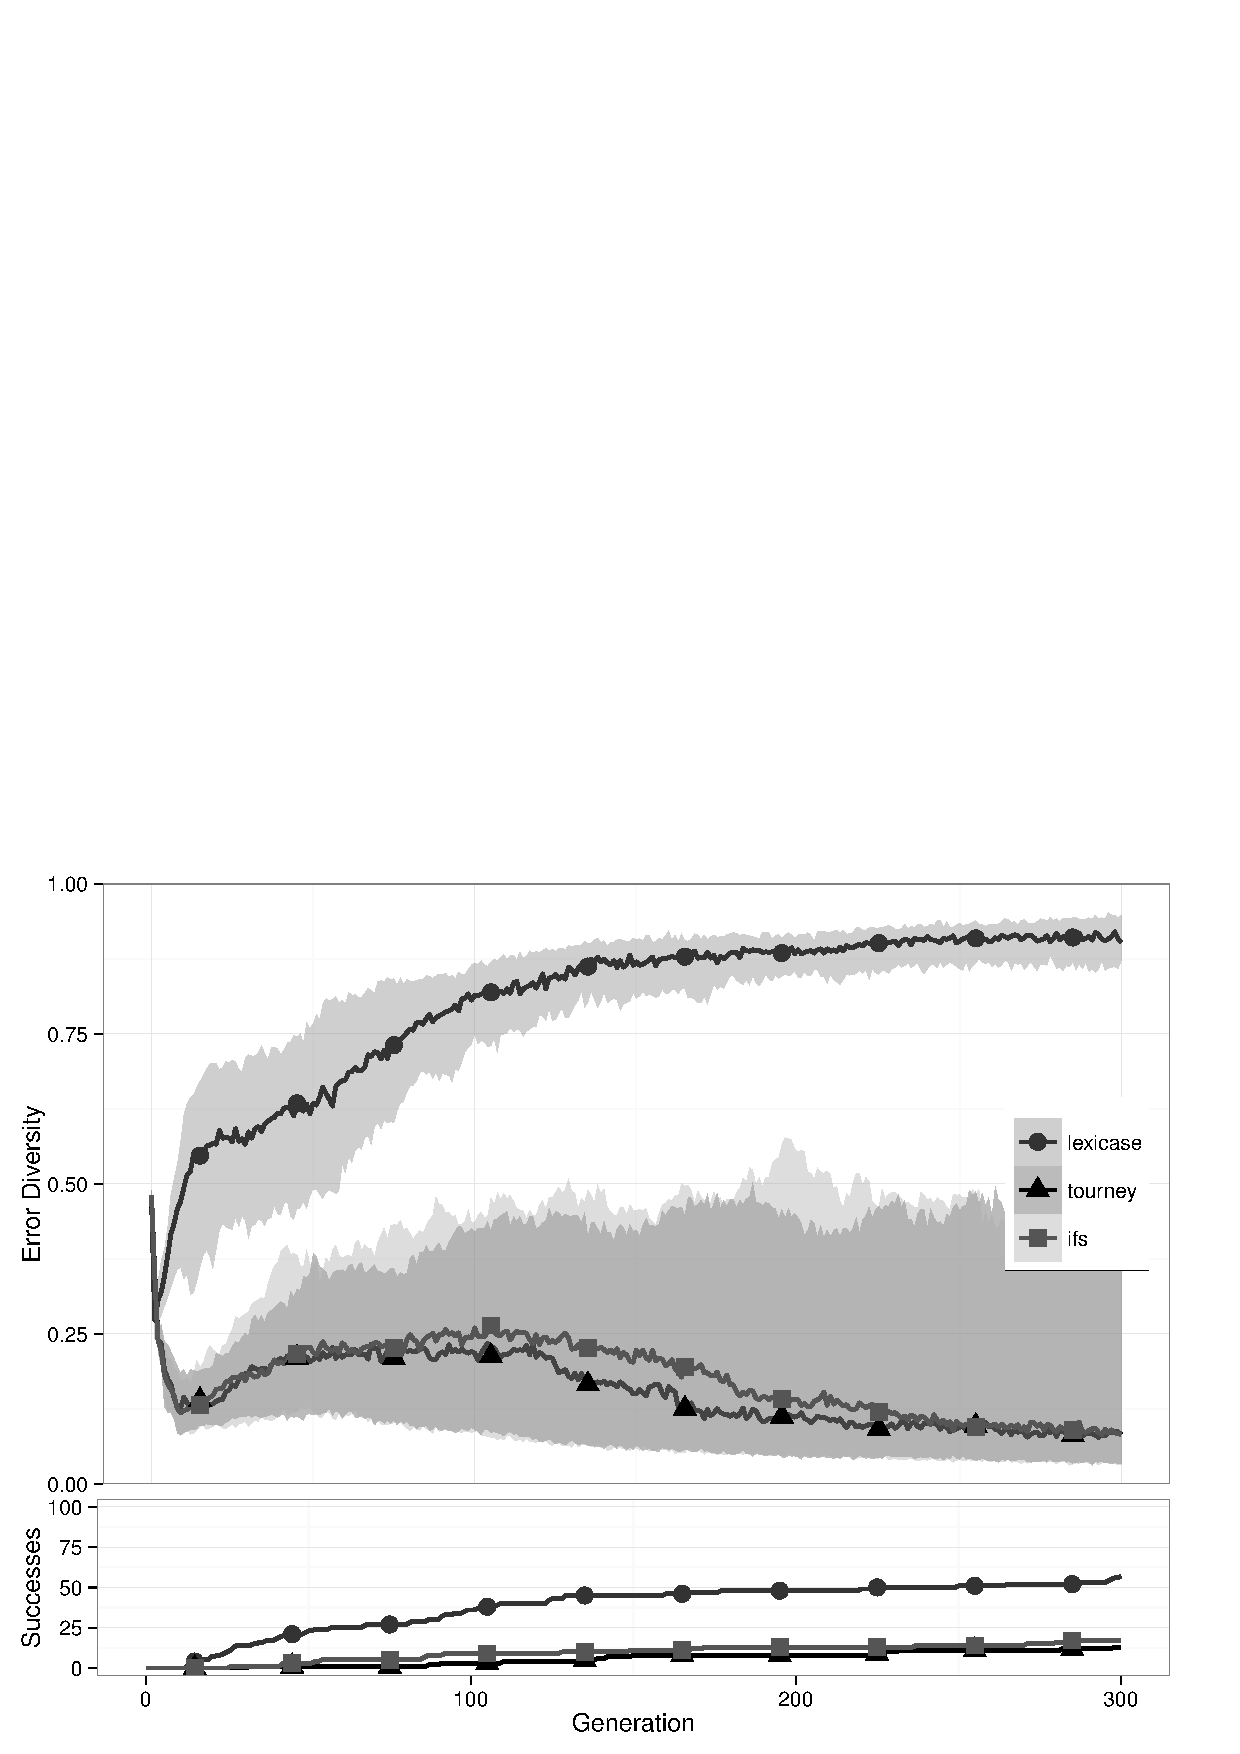
\includegraphics[width=11.5cm]{replace-space-with-newline-diversity.pdf}
\caption{Replace Space With Newline -- error diversity.}
\label{rswnDiv}
\end{figure}

\begin{figure}%[t] %[t] sets the image at the top of the page; t = top, b = bottom, h = here%
%\sidecaption[t]
\centering
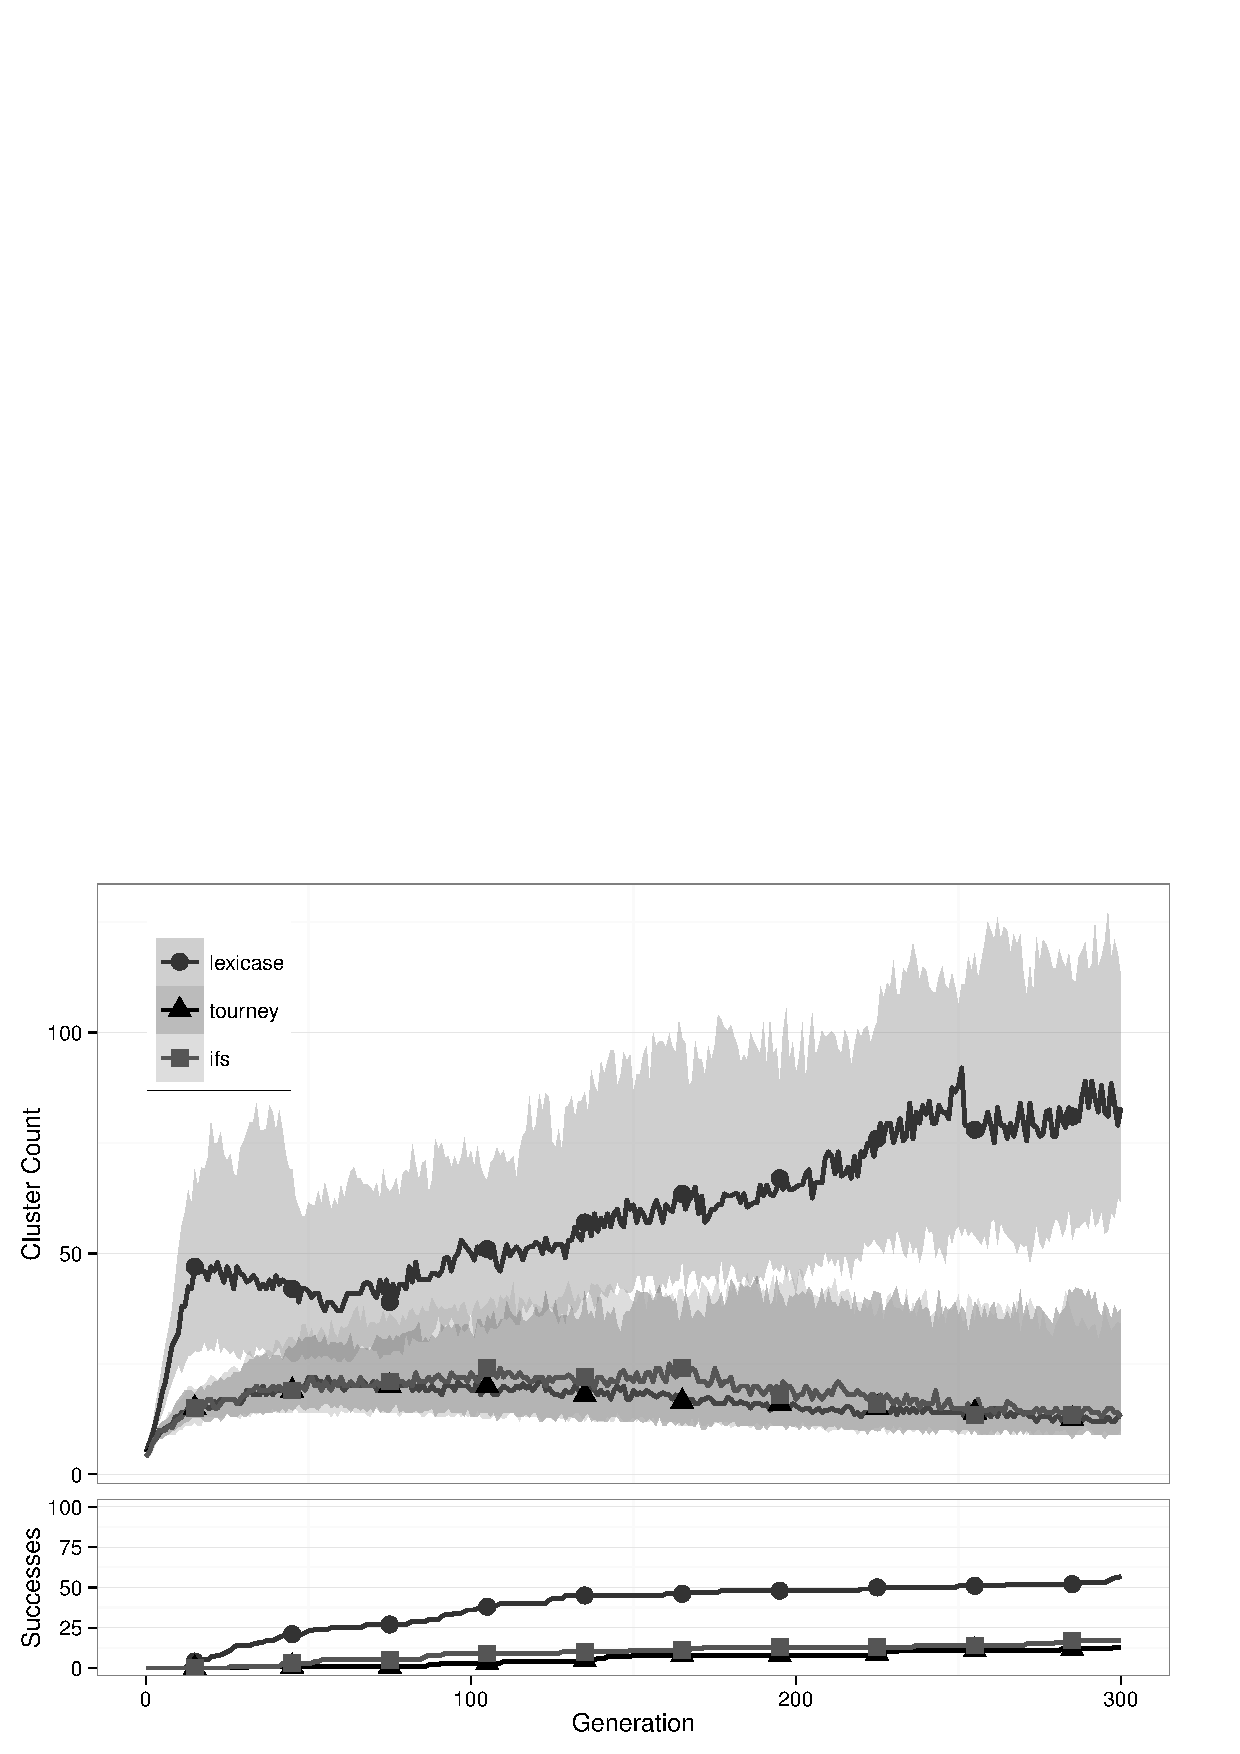
\includegraphics[width=11.5cm]{replace-space-with-newline-cluster.pdf}
\caption{Replace Space With Newline -- clusters.}
\label{rswnClu}
\end{figure}

\begin{figure}%[t] %[t] sets the image at the top of the page; t = top, b = bottom, h = here%
%\sidecaption[t]
\centering
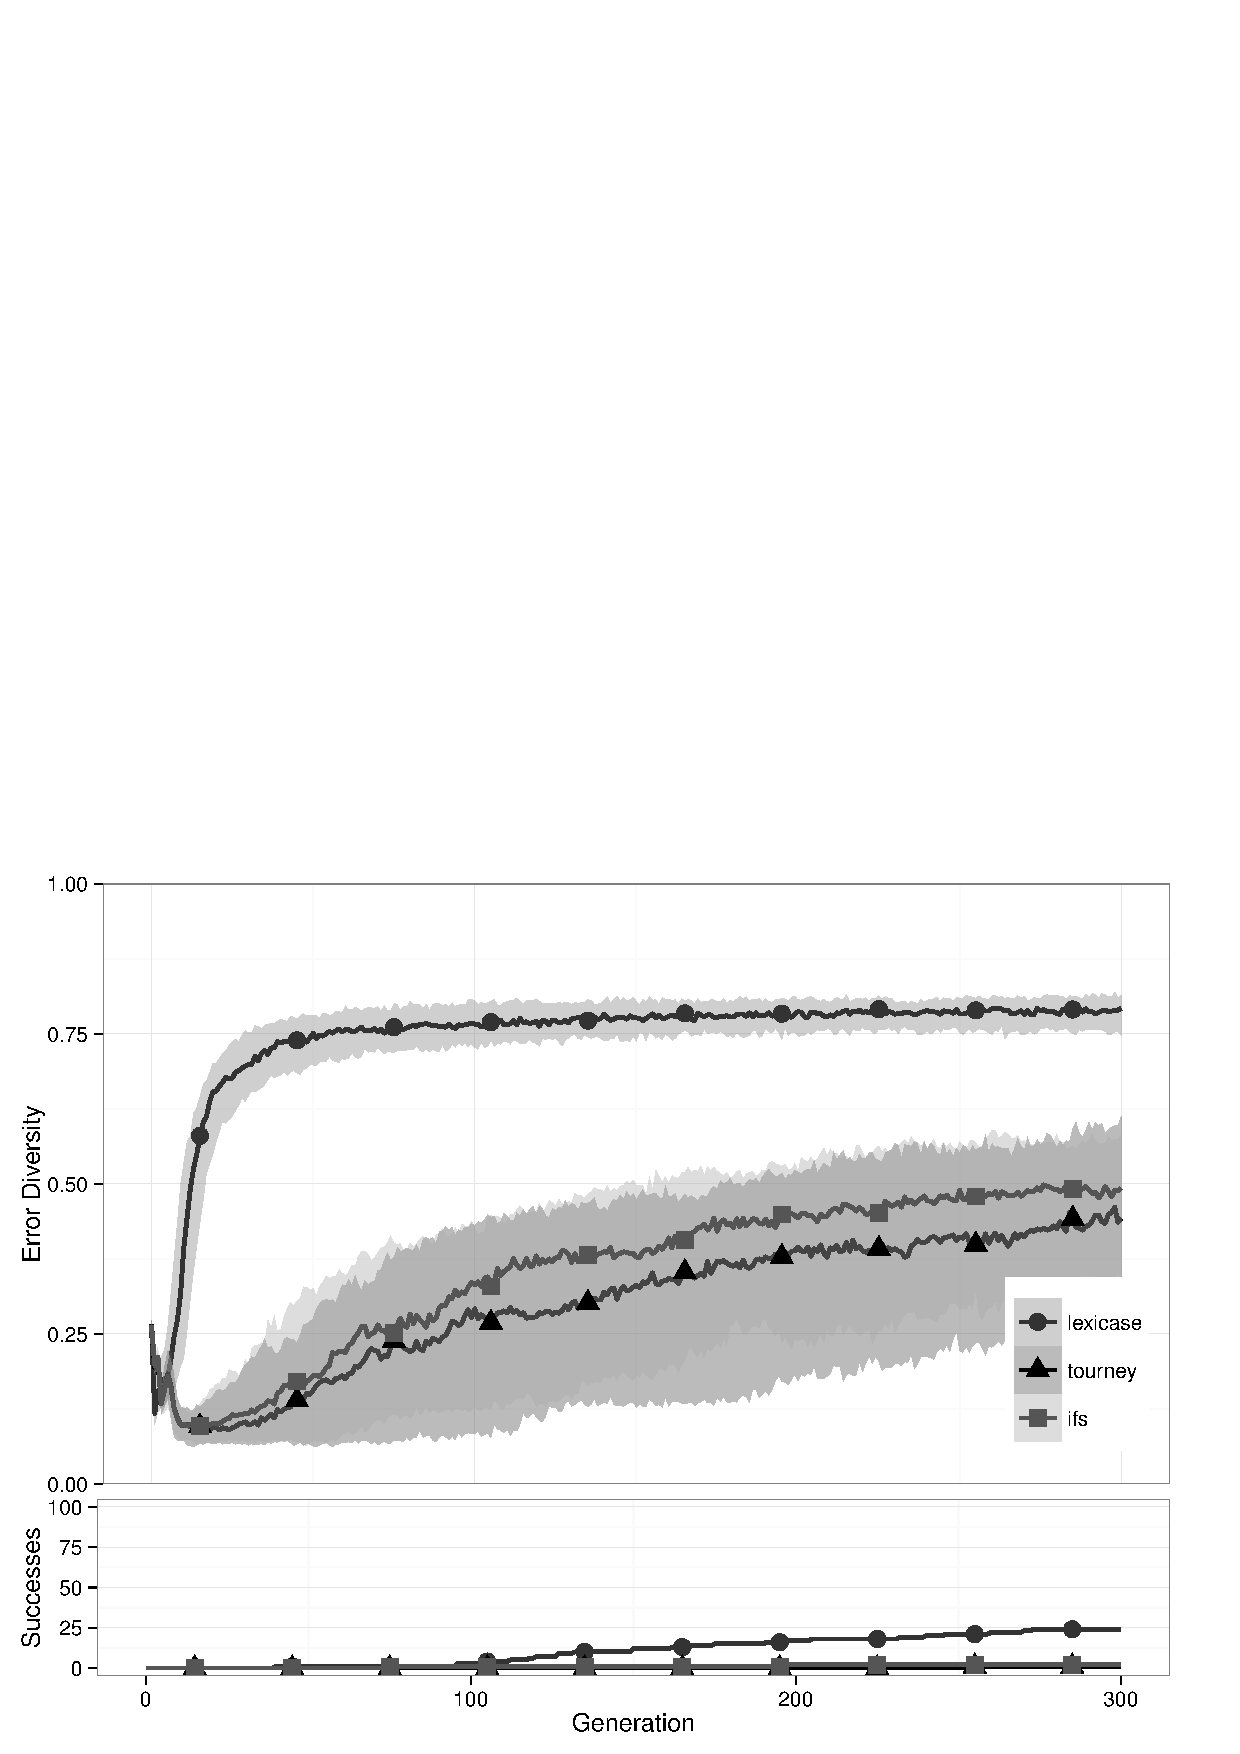
\includegraphics[width=11.5cm]{syllables-diversity.pdf}
\caption{syllables -- error diversity.}
\label{syllablesDiv}
\end{figure}

\begin{figure}%[t] %[t] sets the image at the top of the page; t = top, b = bottom, h = here%
%\sidecaption[t]
\centering
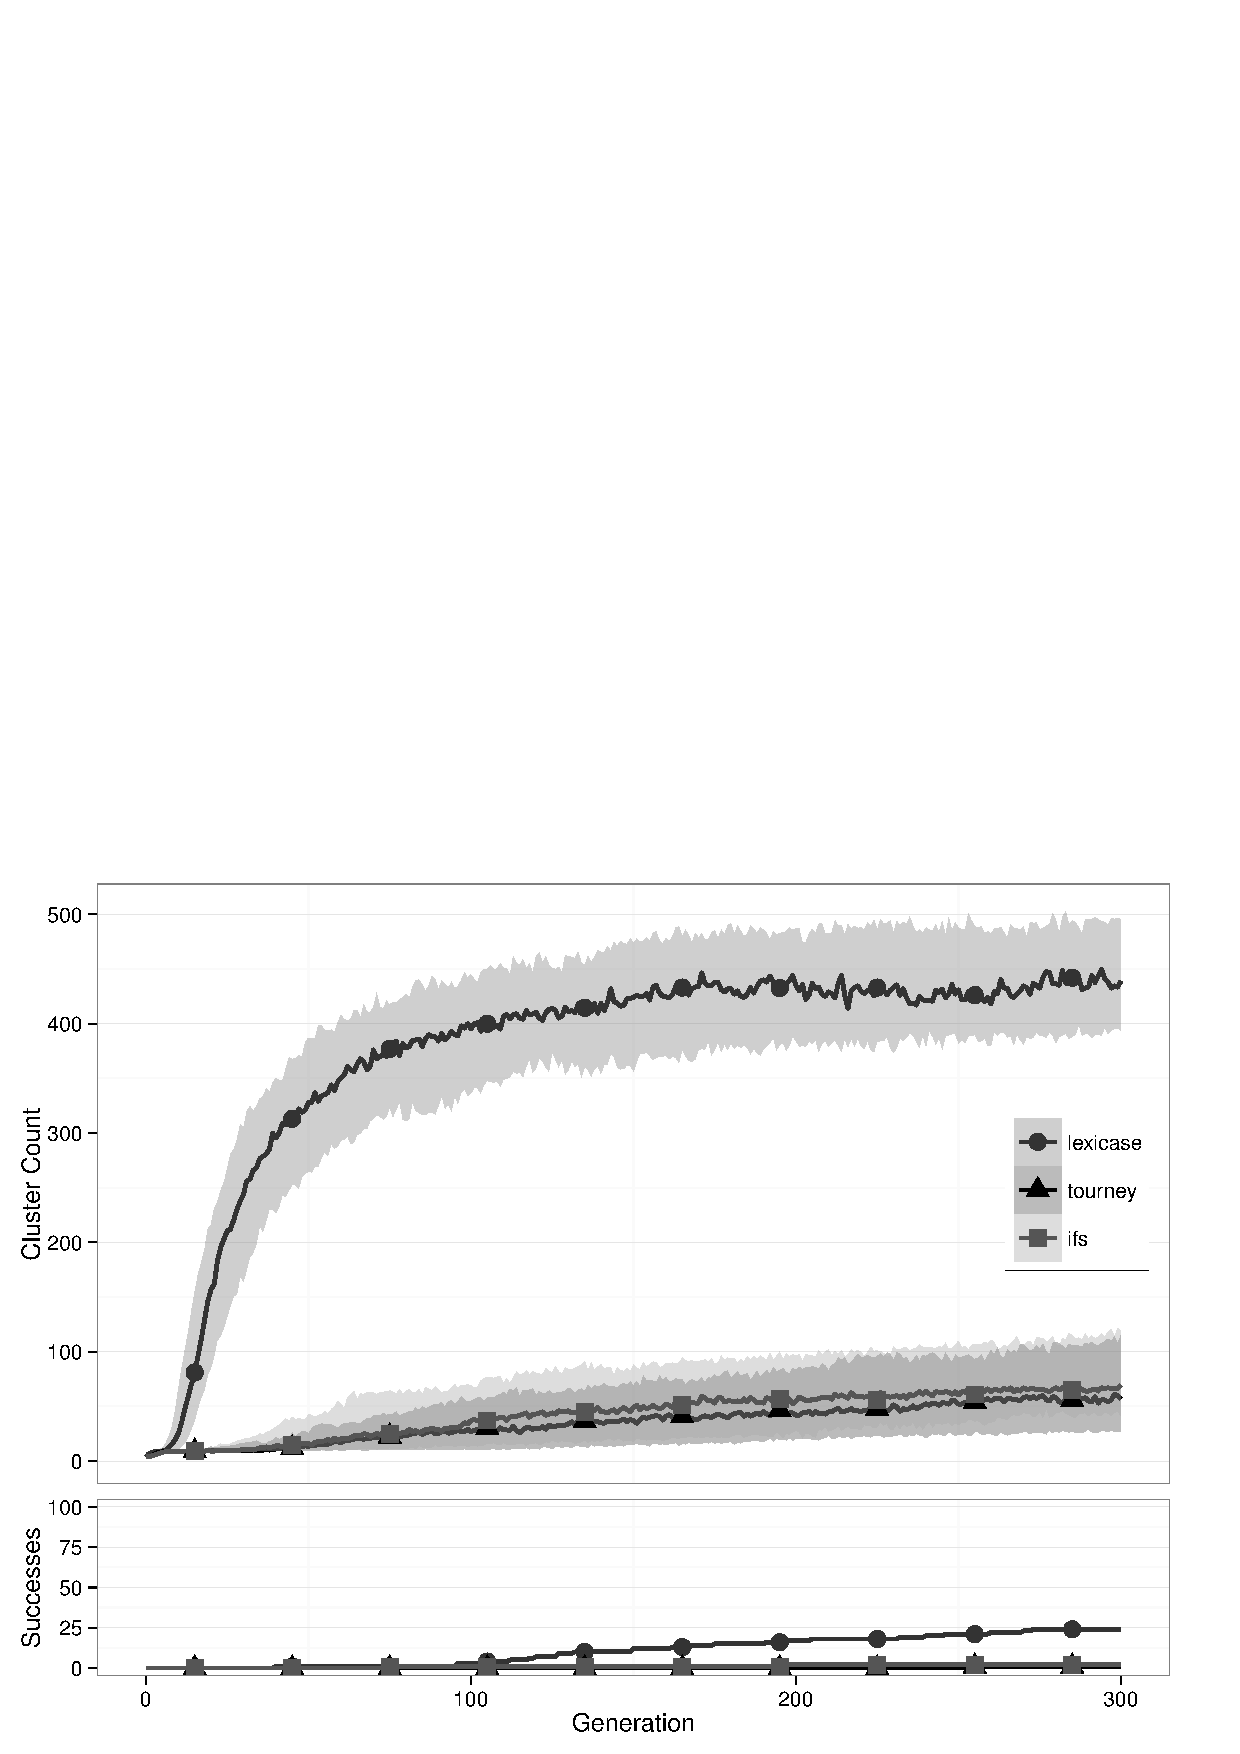
\includegraphics[width=11.5cm]{syllables-cluster.pdf}
\caption{syllables -- clusters.}
\label{syllablesClu}
\end{figure}

\begin{figure}%[t] %[t] sets the image at the top of the page; t = top, b = bottom, h = here%
%\sidecaption[t]
\centering
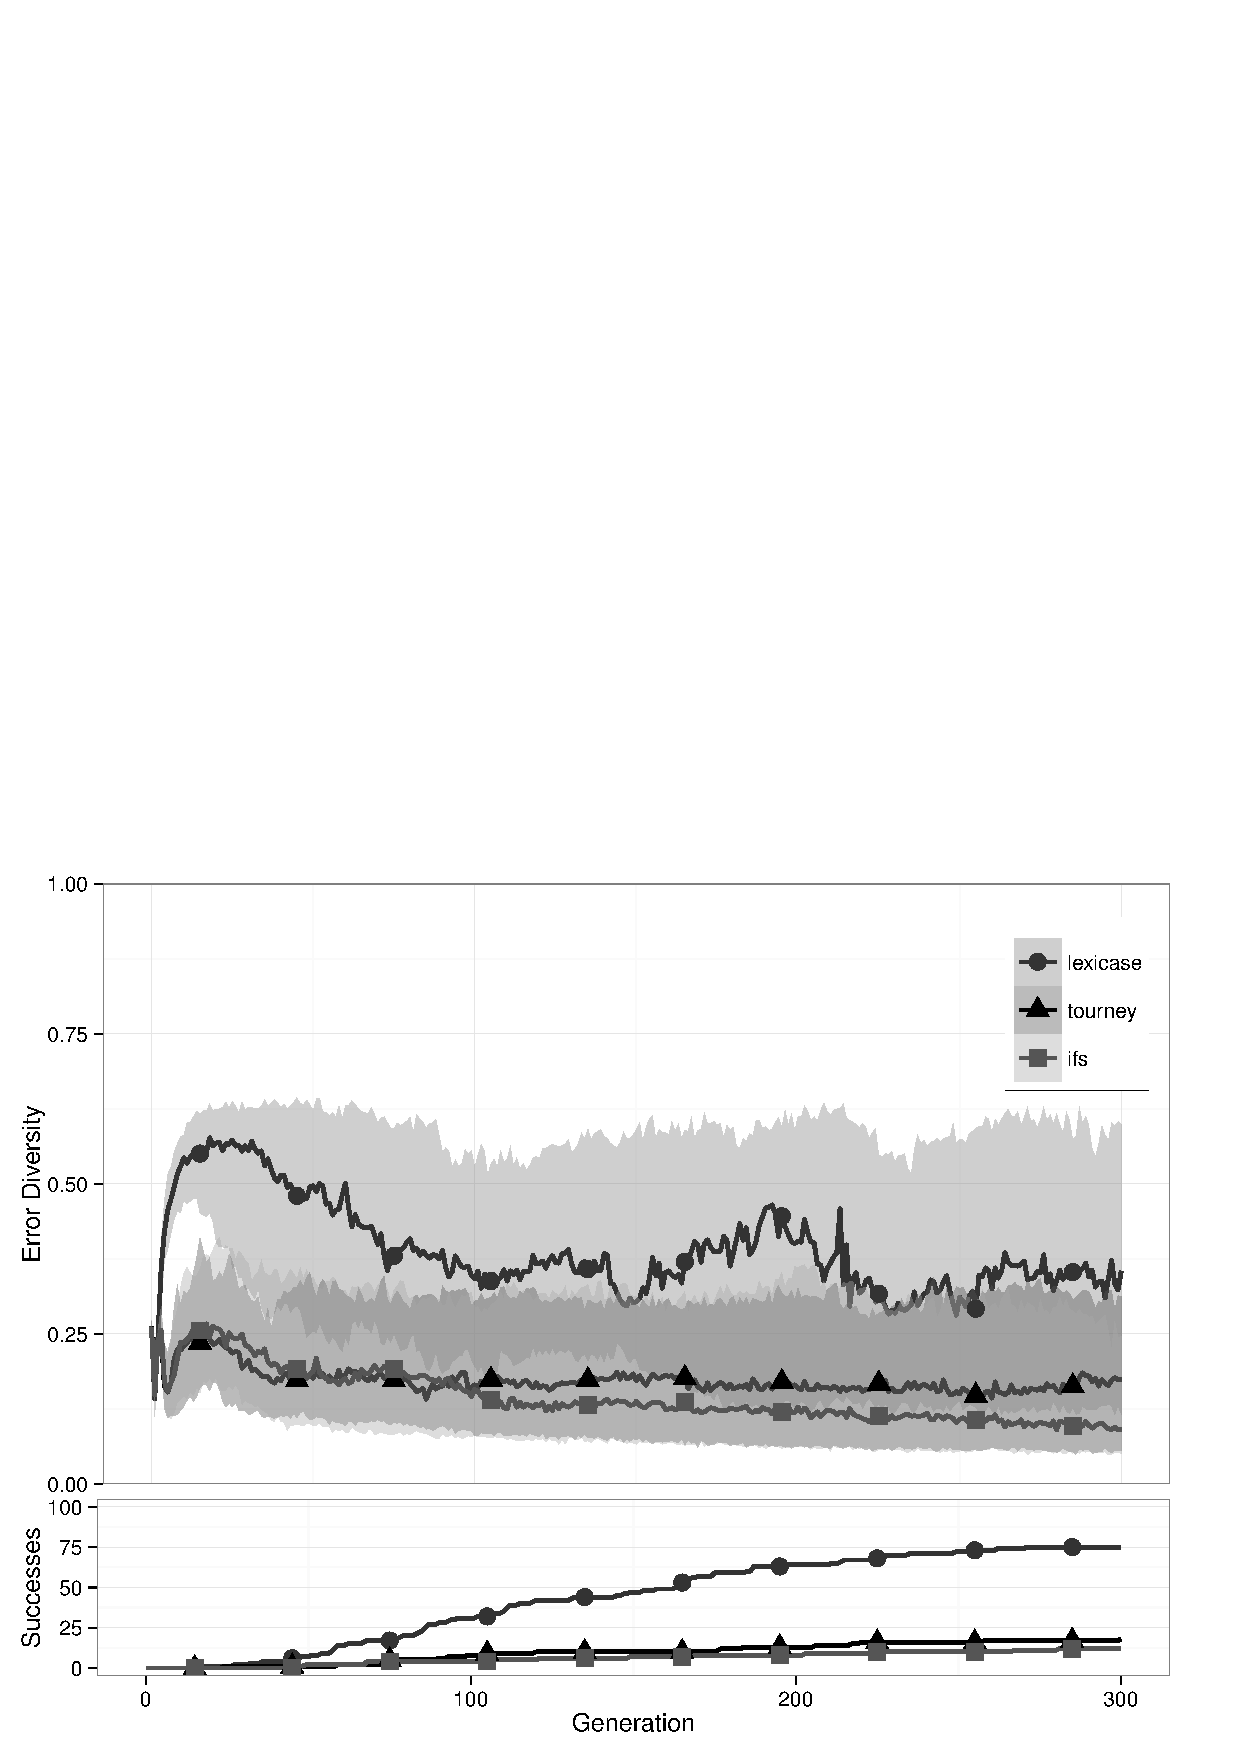
\includegraphics[width=11.5cm]{string-lengths-backwards-diversity.pdf}
\caption{string-lengths-backwards -- error diversity.}
\label{string-lengths-backwardsDiv}
\end{figure}

\begin{figure}%[t] %[t] sets the image at the top of the page; t = top, b = bottom, h = here%
%\sidecaption[t]
\centering
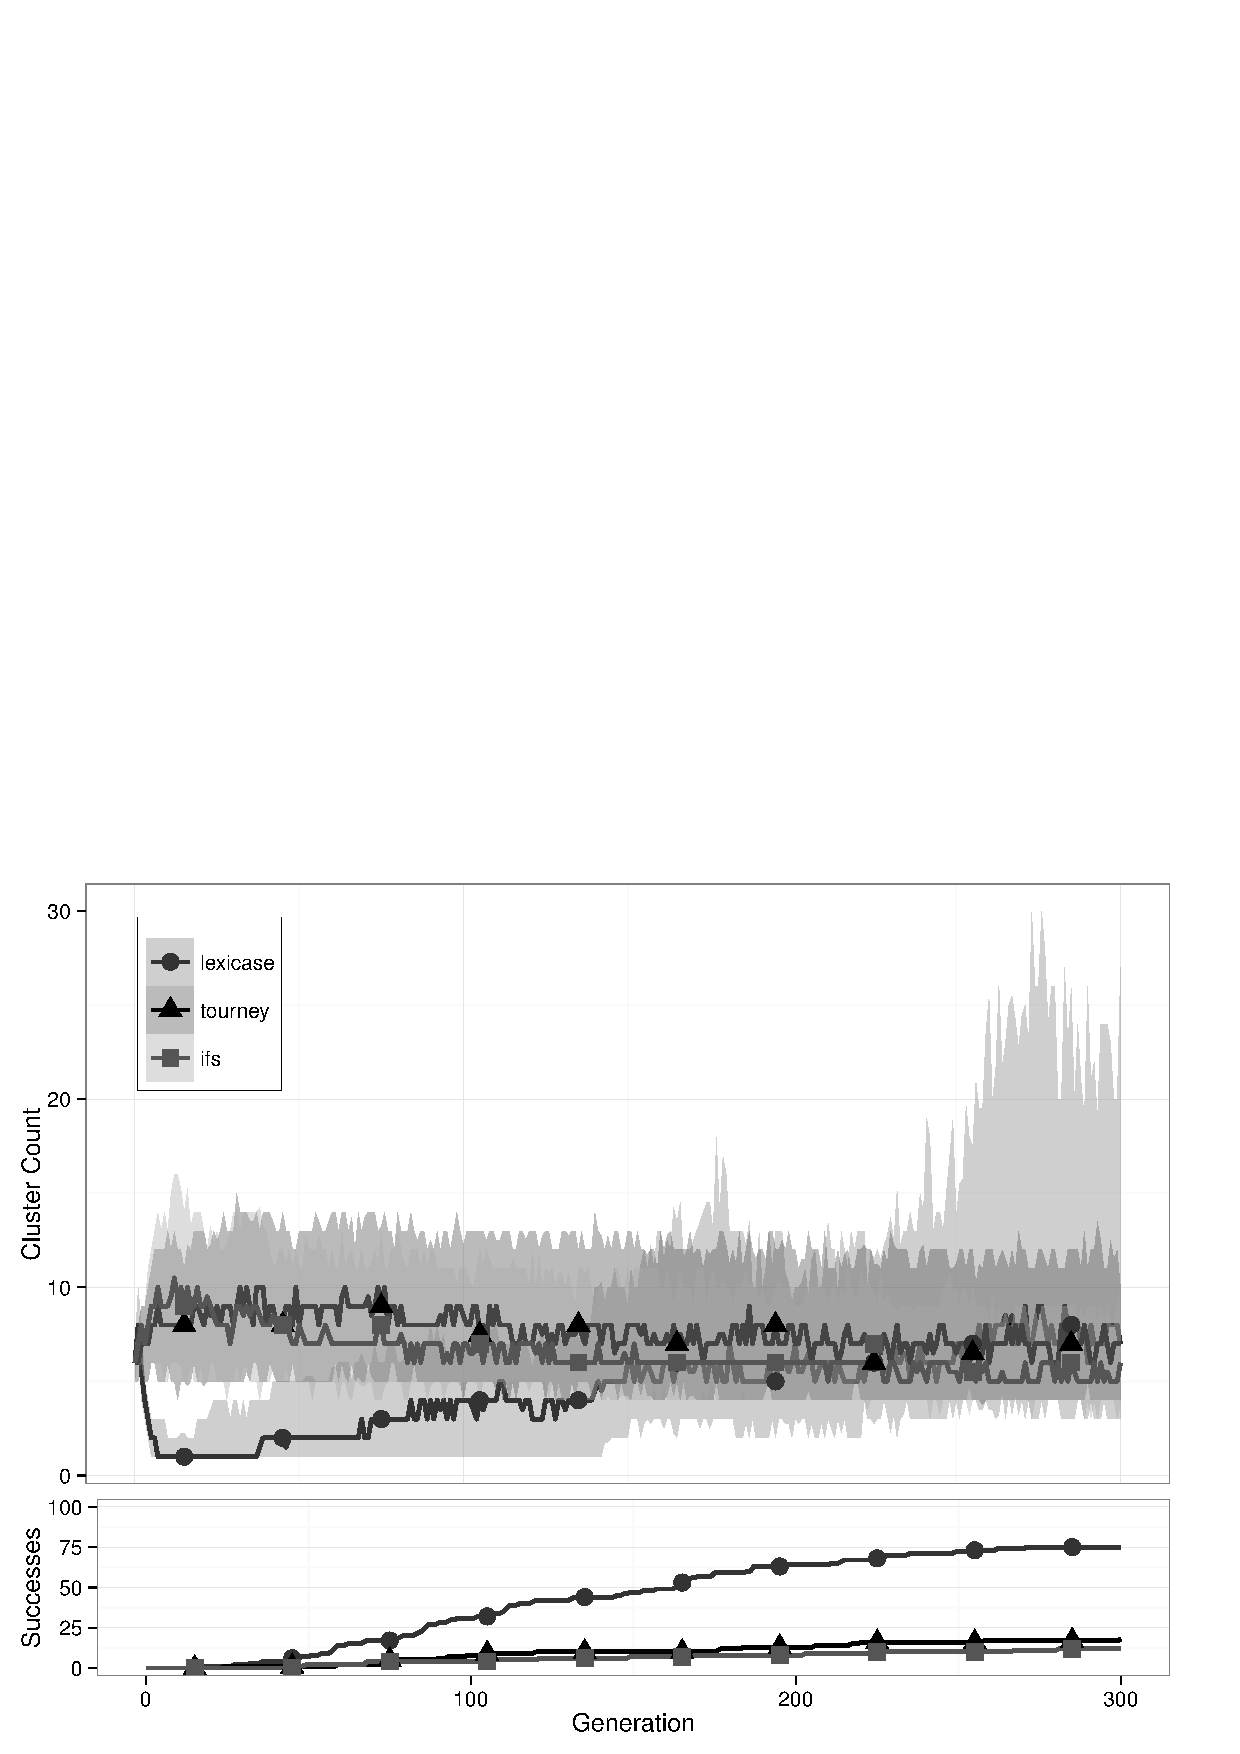
\includegraphics[width=11.5cm]{string-lengths-backwards-cluster.pdf}
\caption{string-lengths-backwards -- clusters.}
\label{string-lengths-backwardsClu}
\end{figure}

\begin{figure}%[t] %[t] sets the image at the top of the page; t = top, b = bottom, h = here%
%\sidecaption[t]
\centering
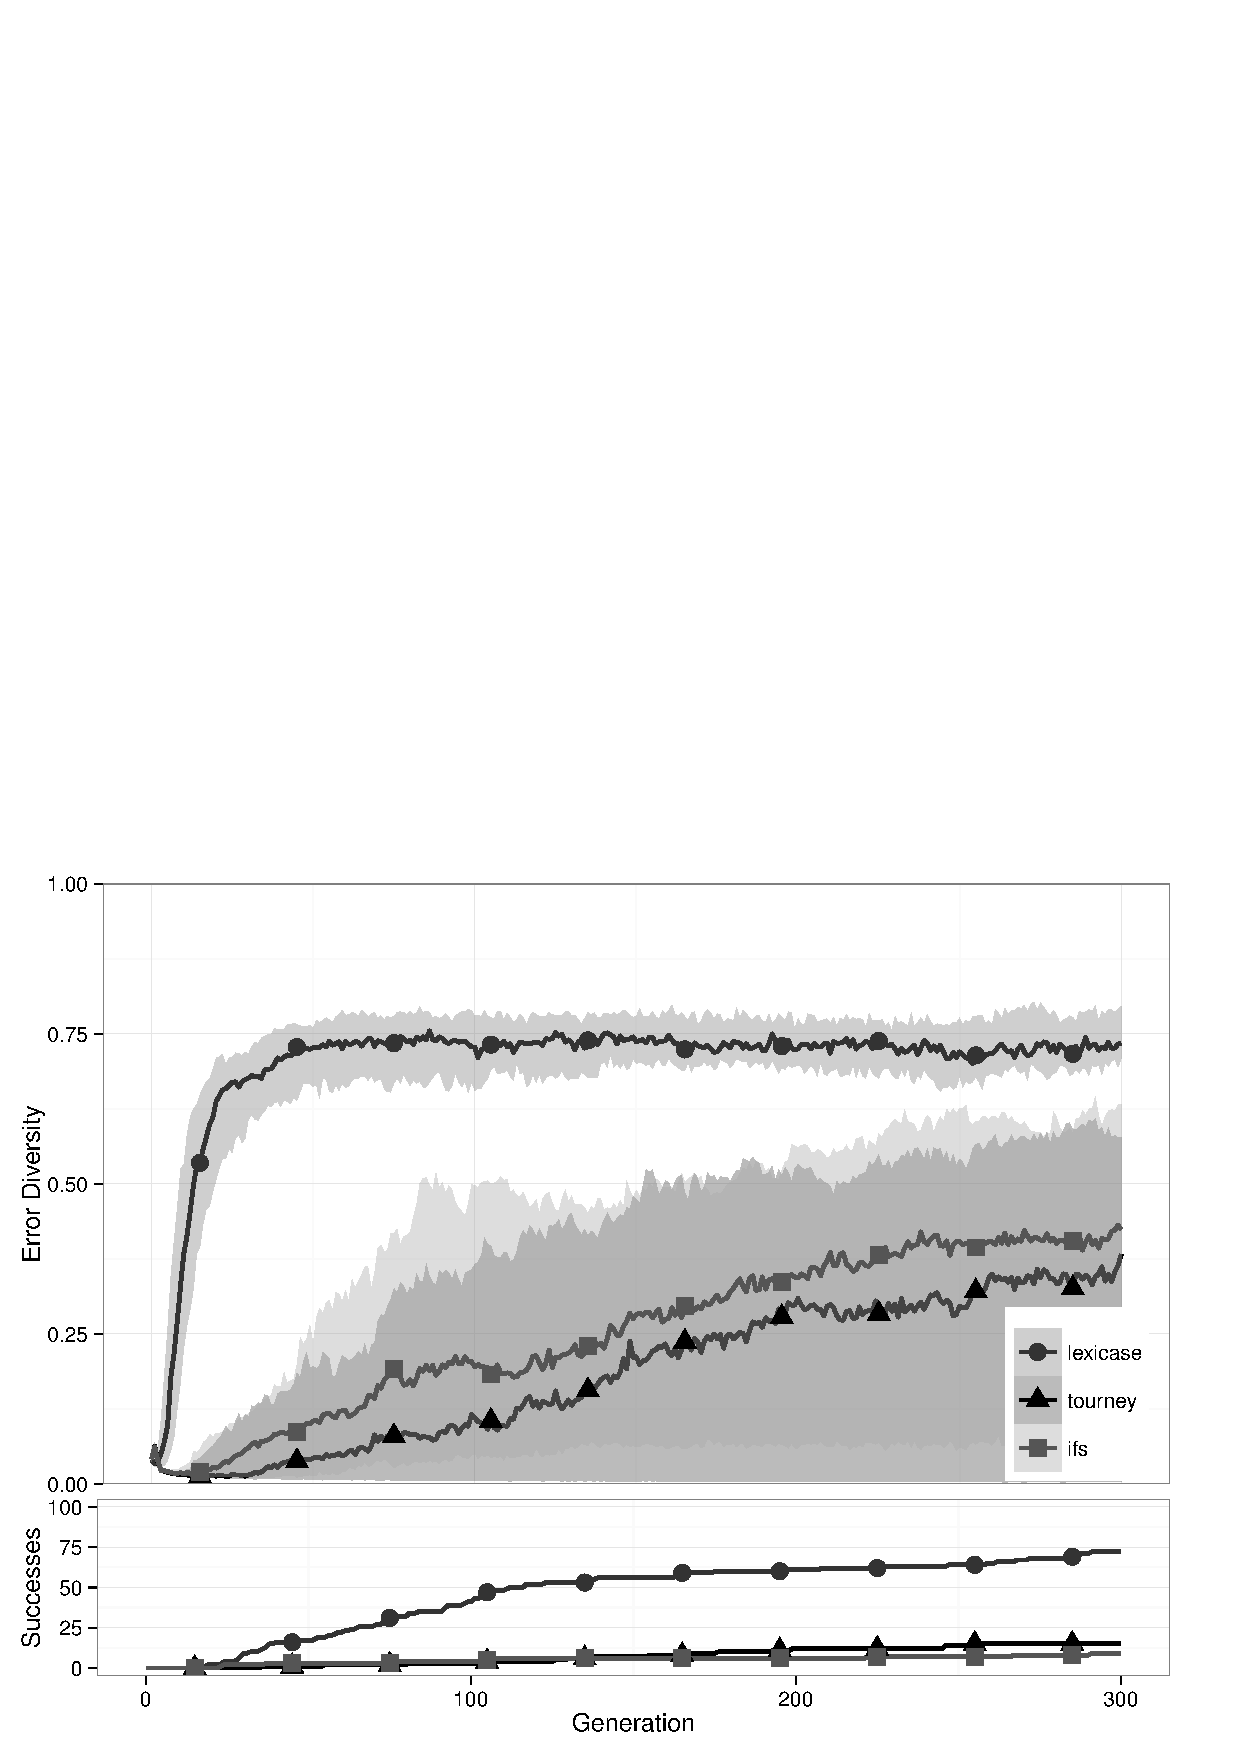
\includegraphics[width=11.5cm]{negative-to-zero-diversity.pdf}
\caption{negative-to-zero -- error diversity.}
\label{negative-to-zeroDiv}
\end{figure}

\begin{figure}%[t] %[t] sets the image at the top of the page; t = top, b = bottom, h = here%
%\sidecaption[t]
\centering
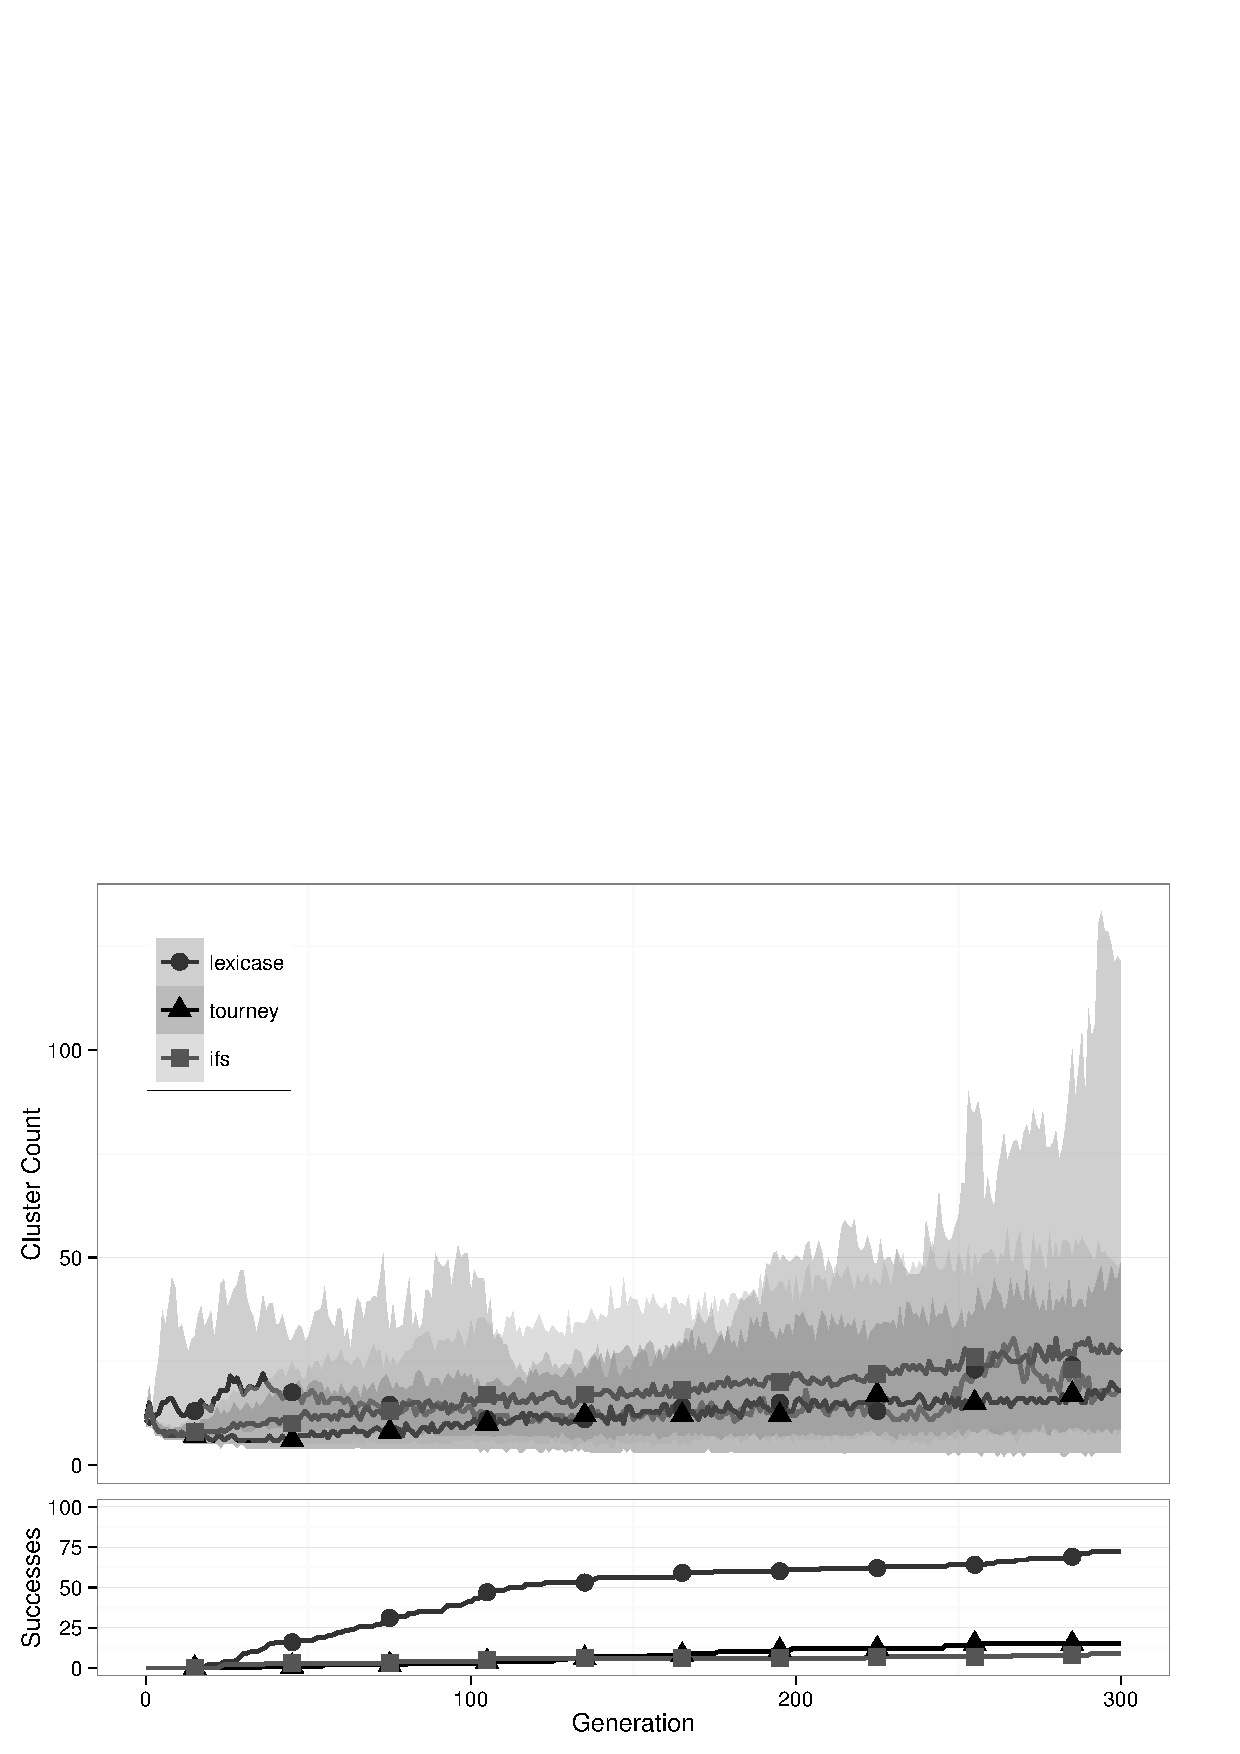
\includegraphics[width=11.5cm]{negative-to-zero-cluster.pdf}
\caption{negative-to-zero -- clusters.}
\label{negative-to-zeroClu}
\end{figure}

\begin{figure}%[t] %[t] sets the image at the top of the page; t = top, b = bottom, h = here%
%\sidecaption[t]
\centering
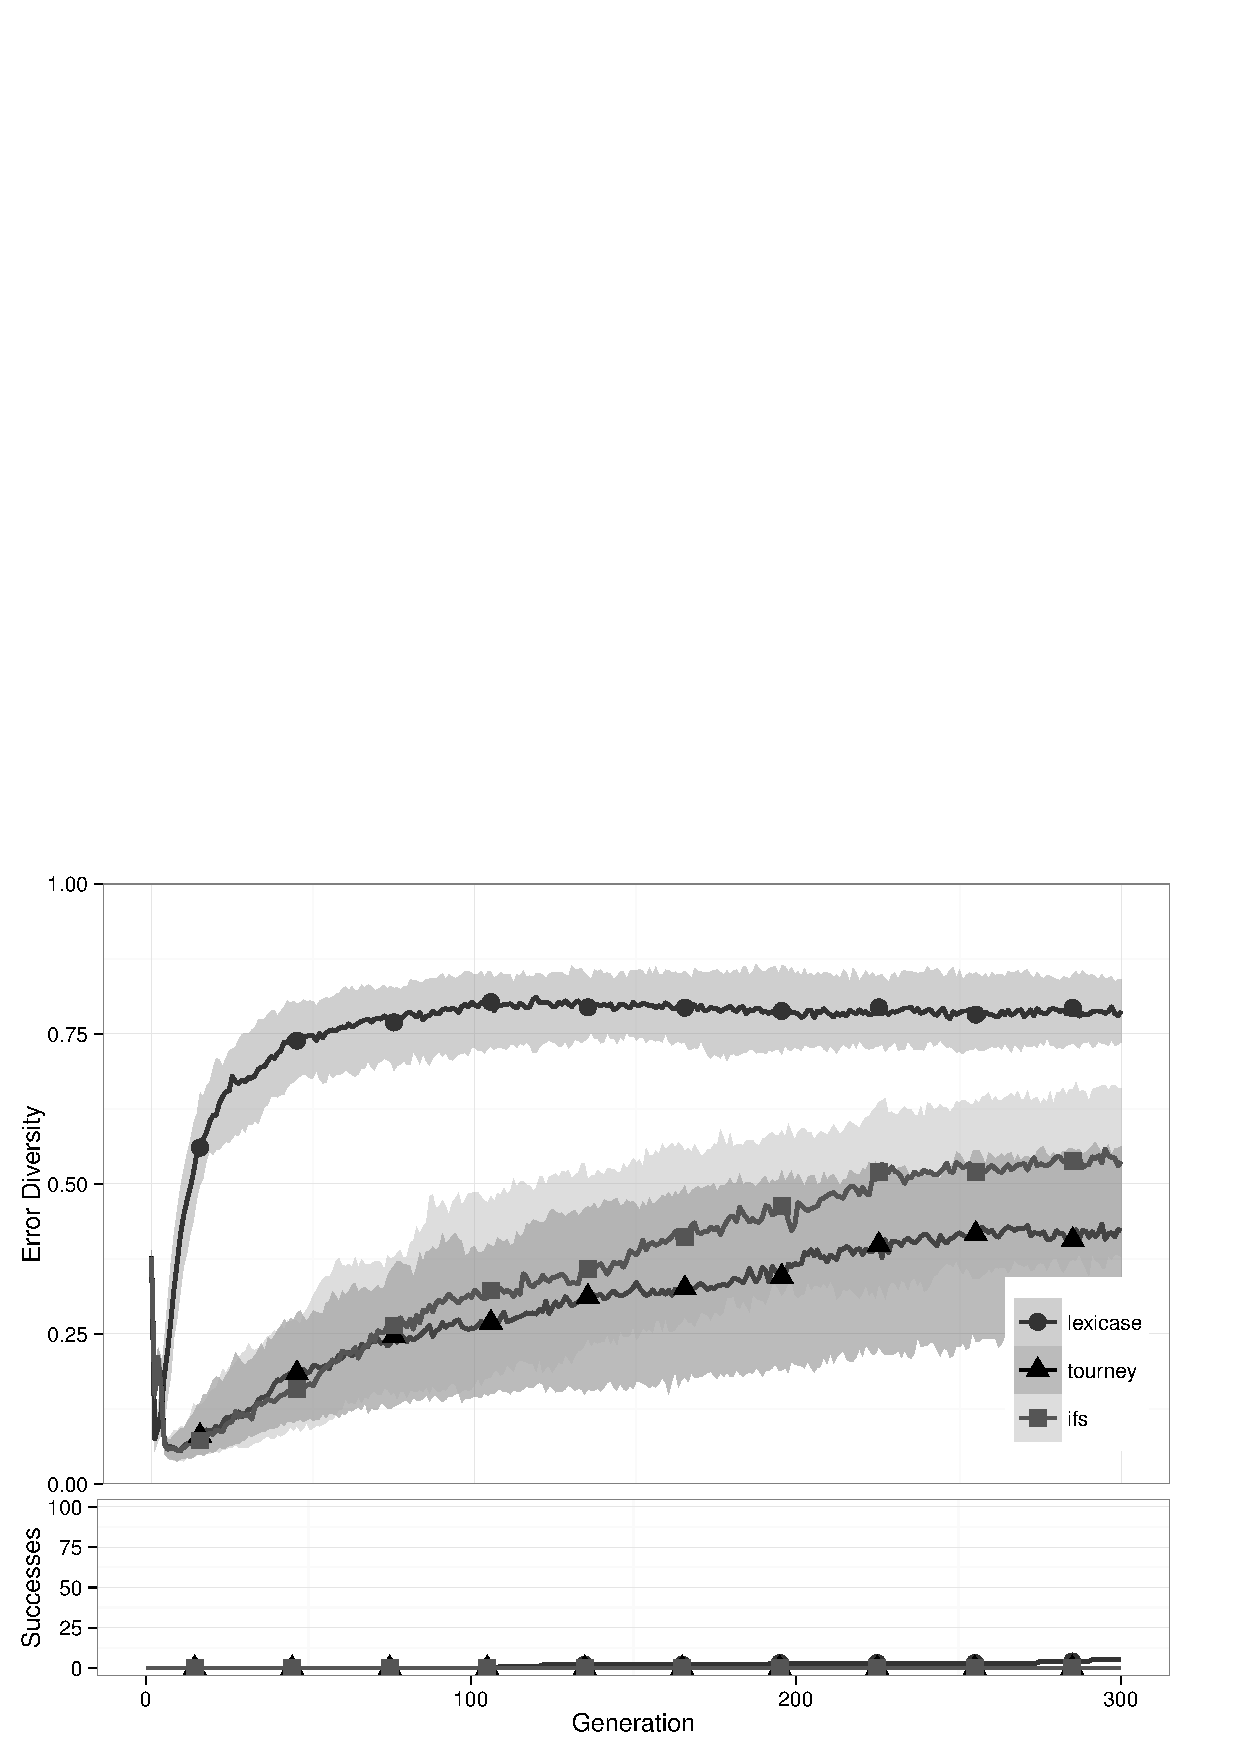
\includegraphics[width=11.5cm]{double-letters-diversity.pdf}
\caption{double-letters -- error diversity.}
\label{double-lettersDiv}
\end{figure}

\begin{figure}%[t] %[t] sets the image at the top of the page; t = top, b = bottom, h = here%
%\sidecaption[t]
\centering
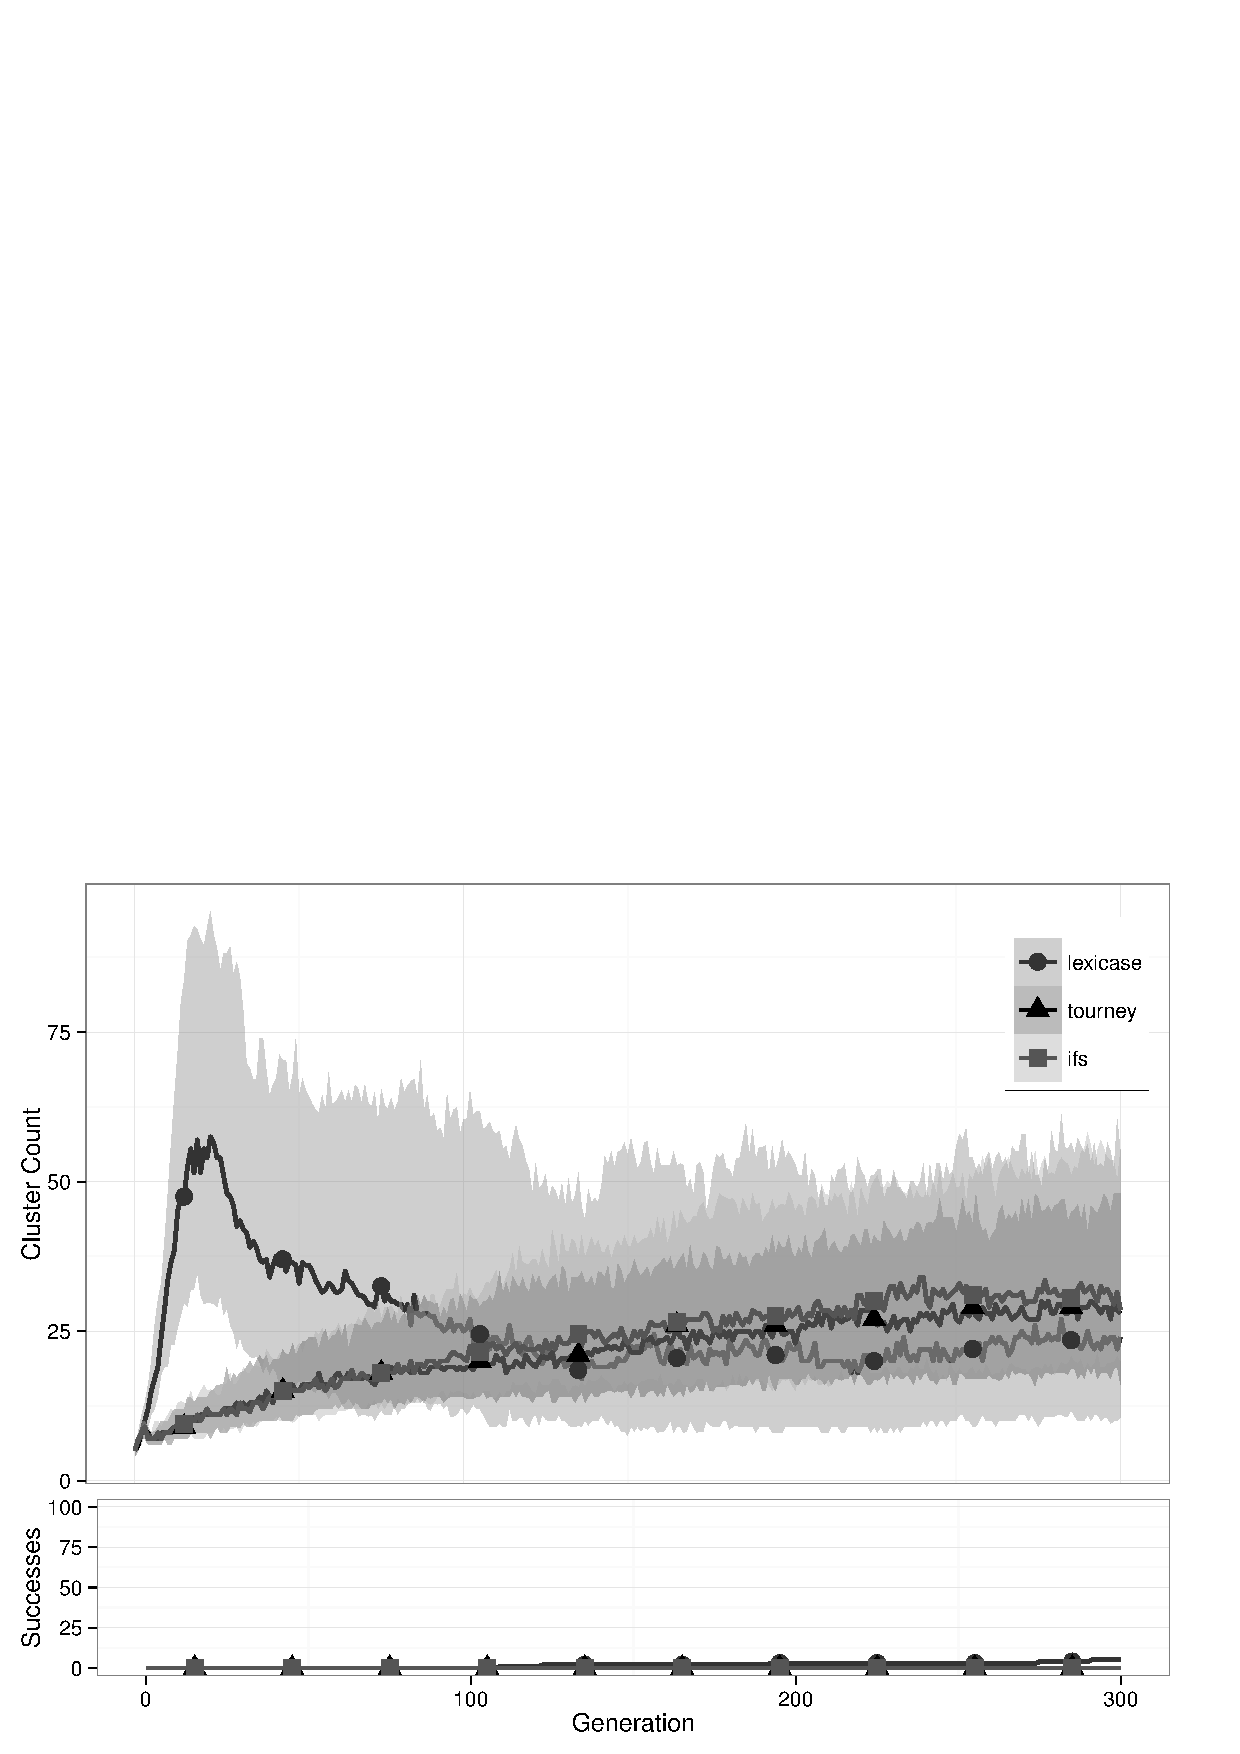
\includegraphics[width=11.5cm]{double-letters-cluster.pdf}
\caption{double-letters -- clusters.}
\label{double-lettersClu}
\end{figure}

\begin{figure}%[t] %[t] sets the image at the top of the page; t = top, b = bottom, h = here%
%\sidecaption[t]
\centering
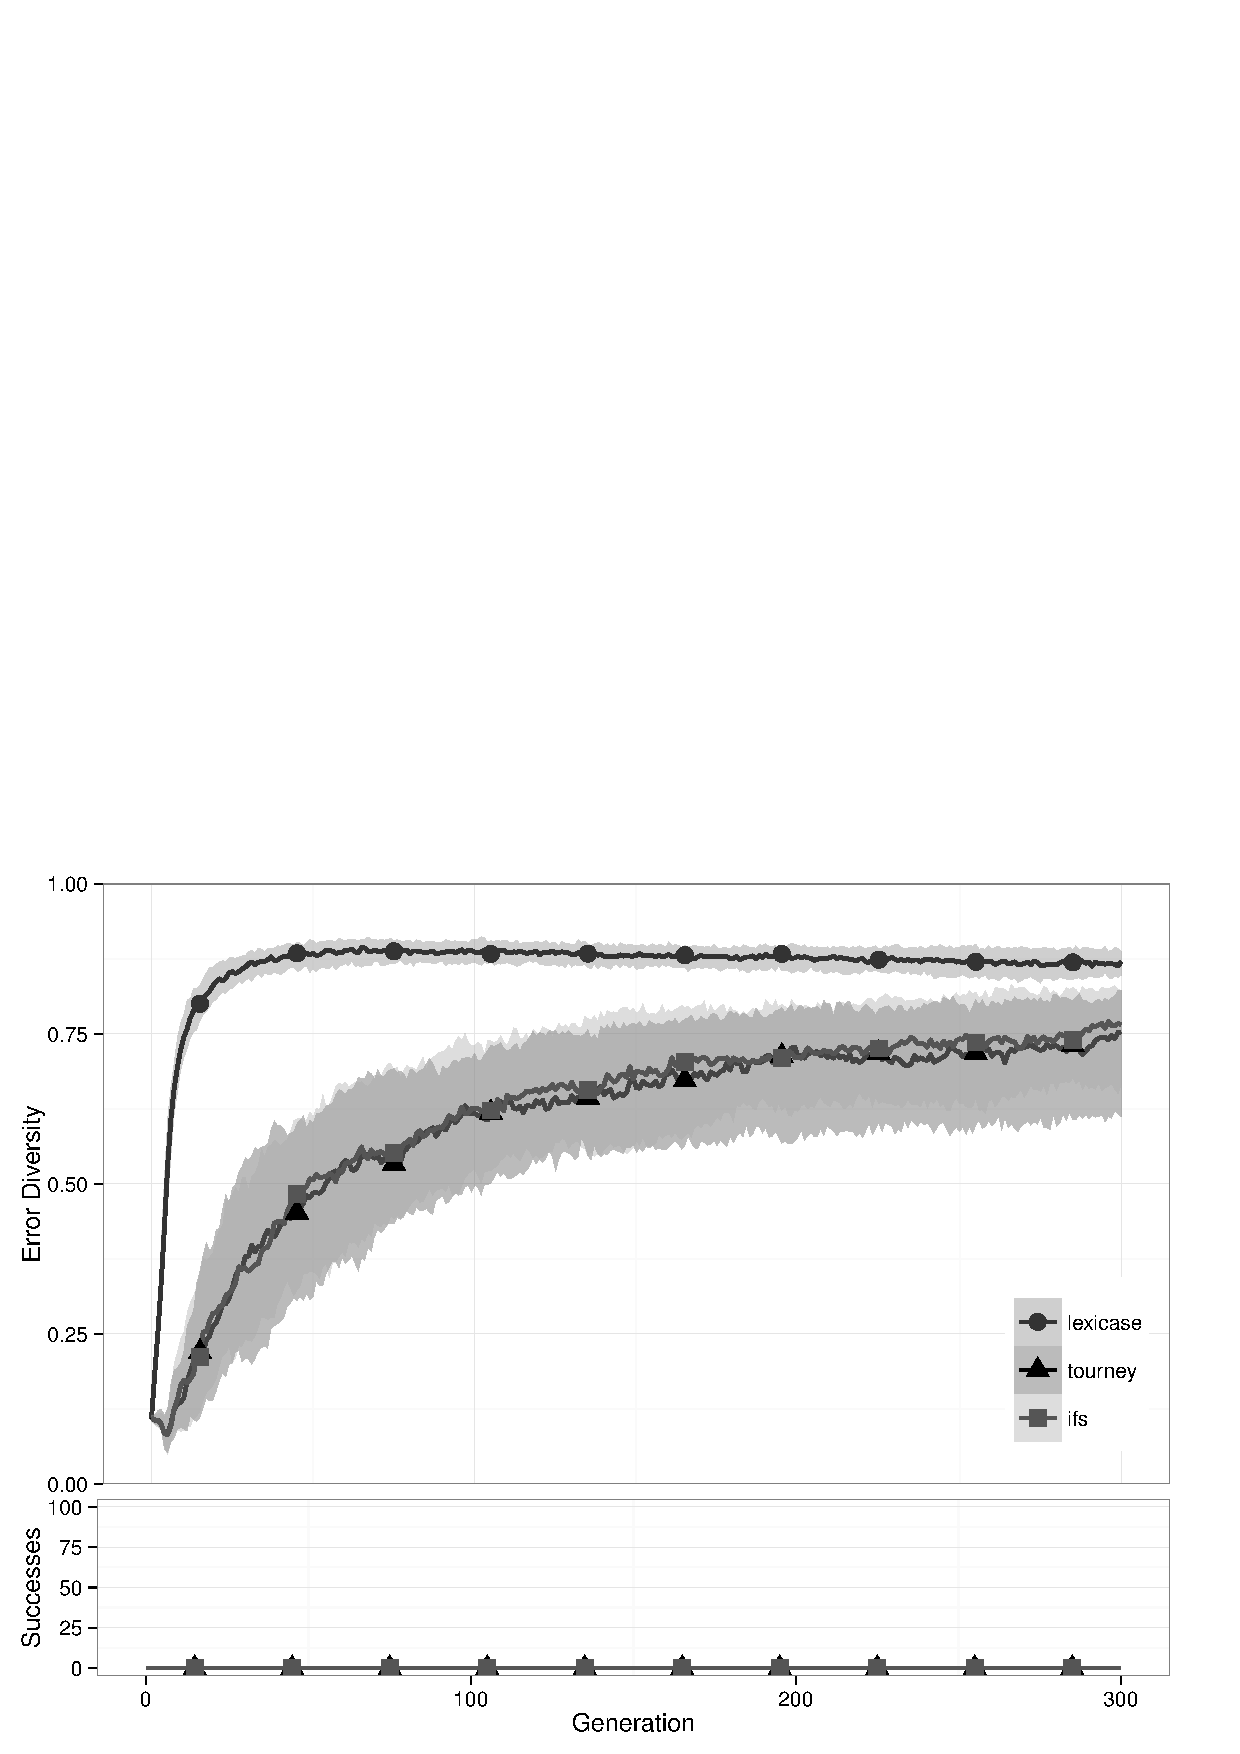
\includegraphics[width=11.5cm]{scrabble-score-diversity.pdf}
\caption{scrabble-score -- error diversity.}
\label{scrabble-scoreDiv}
\end{figure}

\begin{figure}%[t] %[t] sets the image at the top of the page; t = top, b = bottom, h = here%
%\sidecaption[t]
\centering
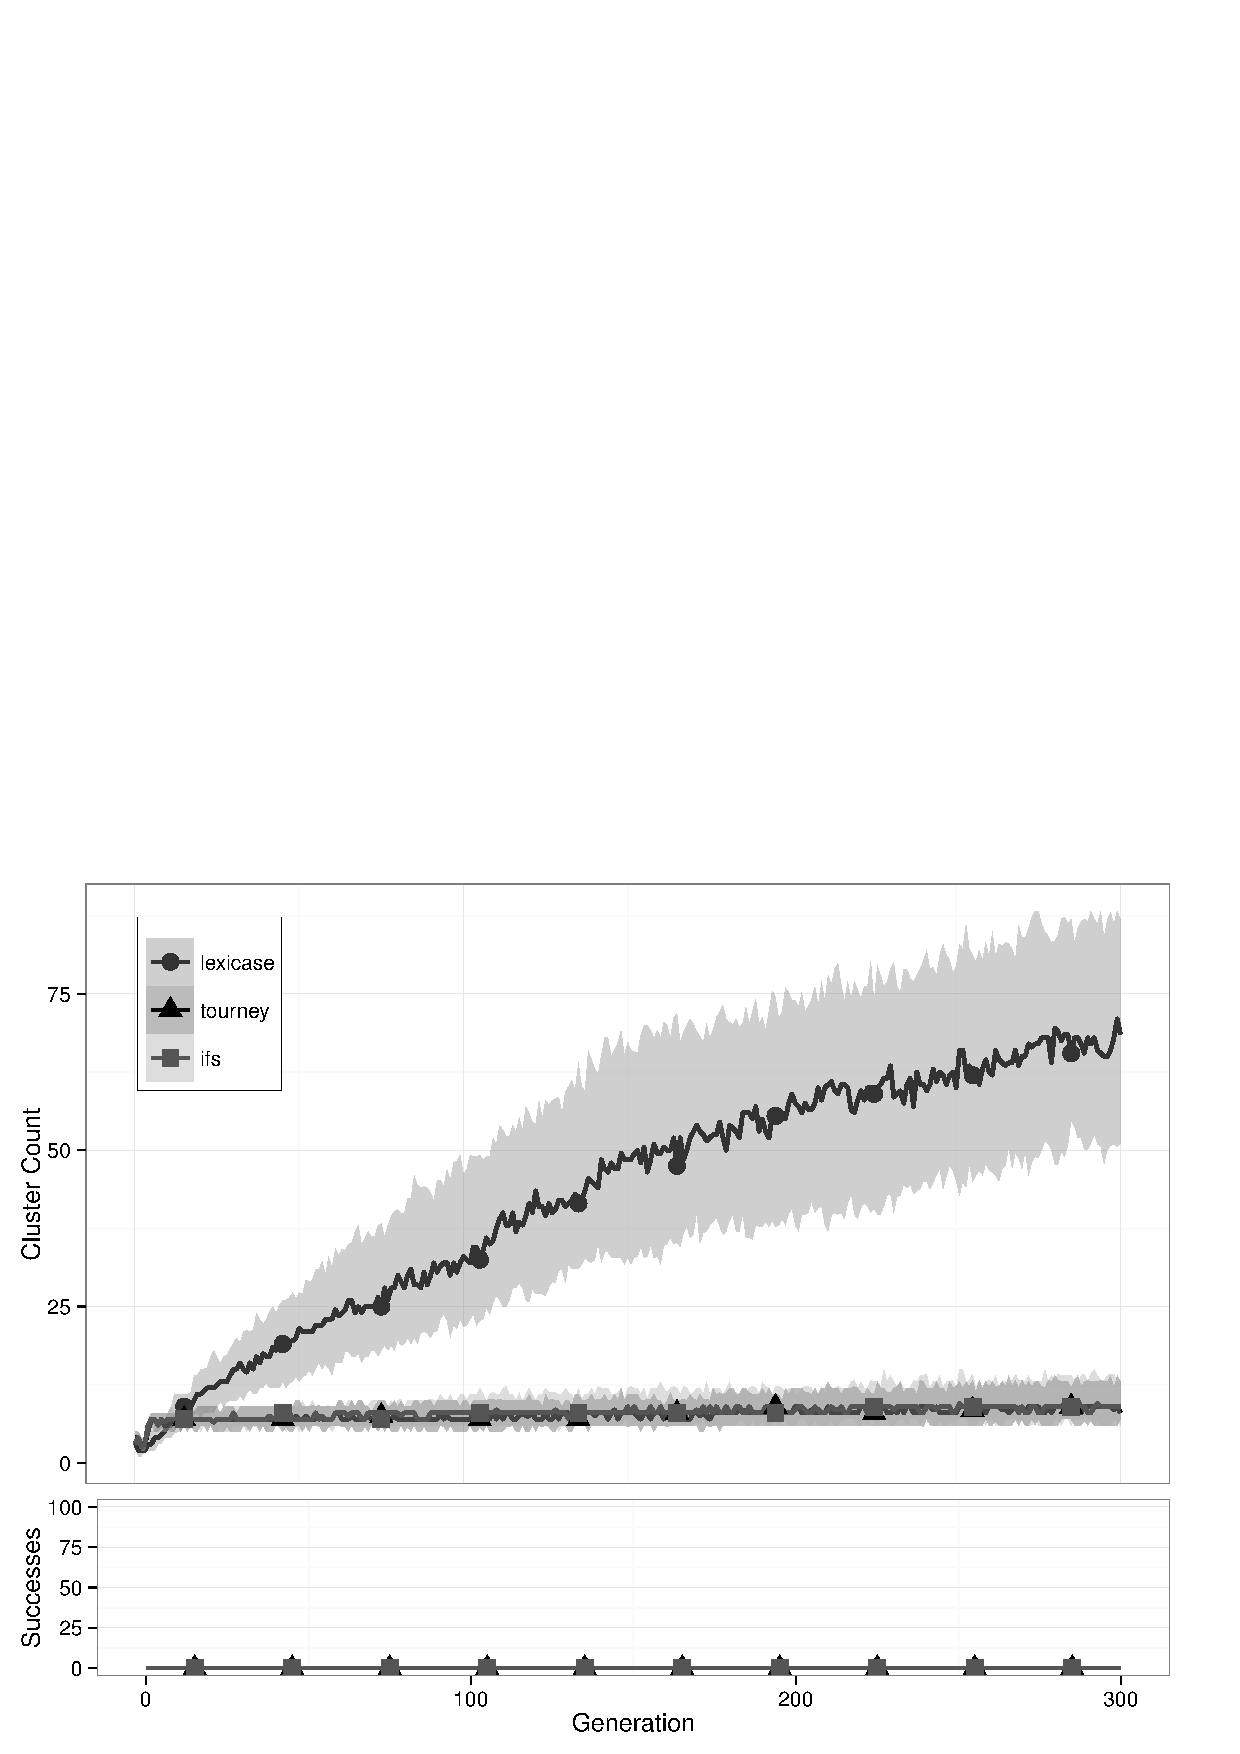
\includegraphics[width=11.5cm]{scrabble-score-cluster.pdf}
\caption{scrabble-score -- clusters.}
\label{scrabble-scoreClu}
\end{figure}

\begin{figure}%[t] %[t] sets the image at the top of the page; t = top, b = bottom, h = here%
%\sidecaption[t]
\centering
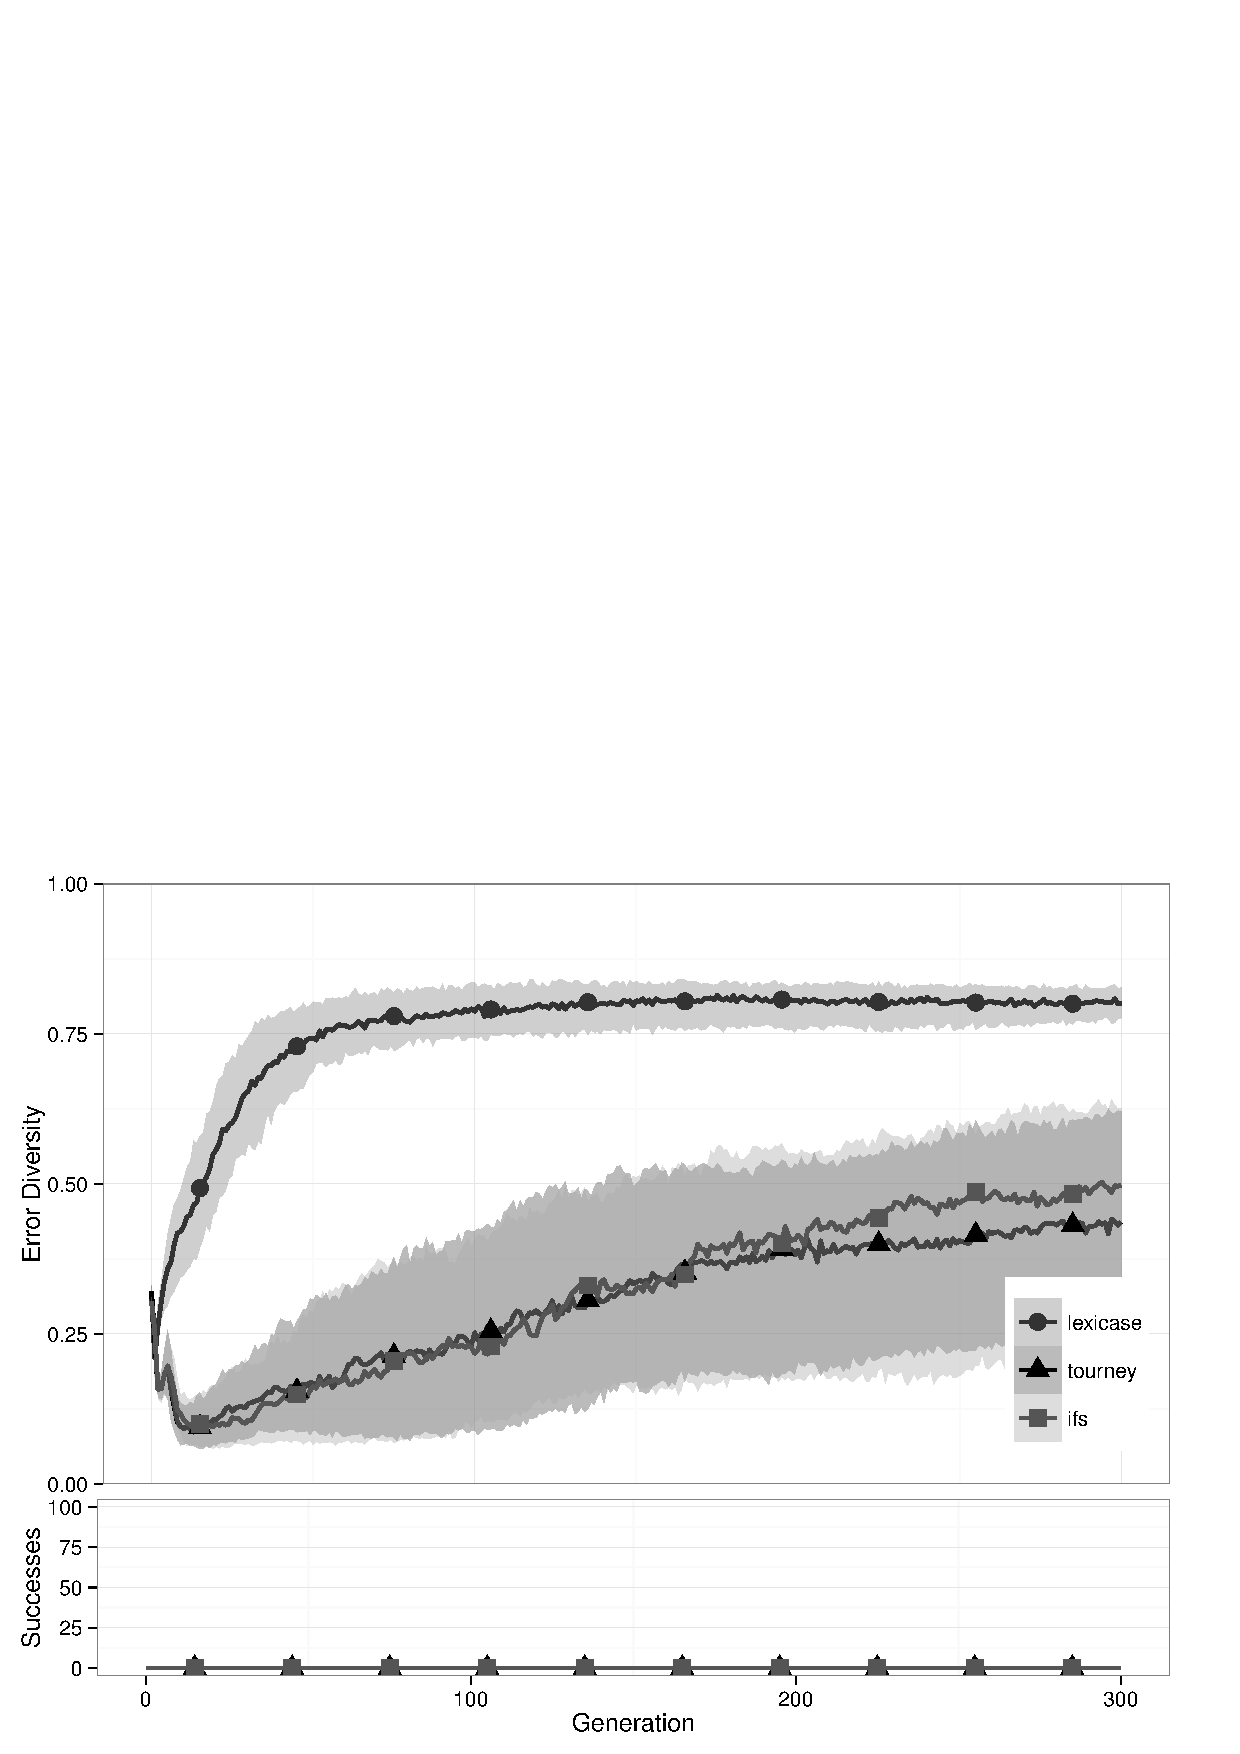
\includegraphics[width=11.5cm]{checksum-diversity.pdf}
\caption{checksum -- error diversity.}
\label{checksumDiv}
\end{figure}

\begin{figure}%[t] %[t] sets the image at the top of the page; t = top, b = bottom, h = here%
%\sidecaption[t]
\centering
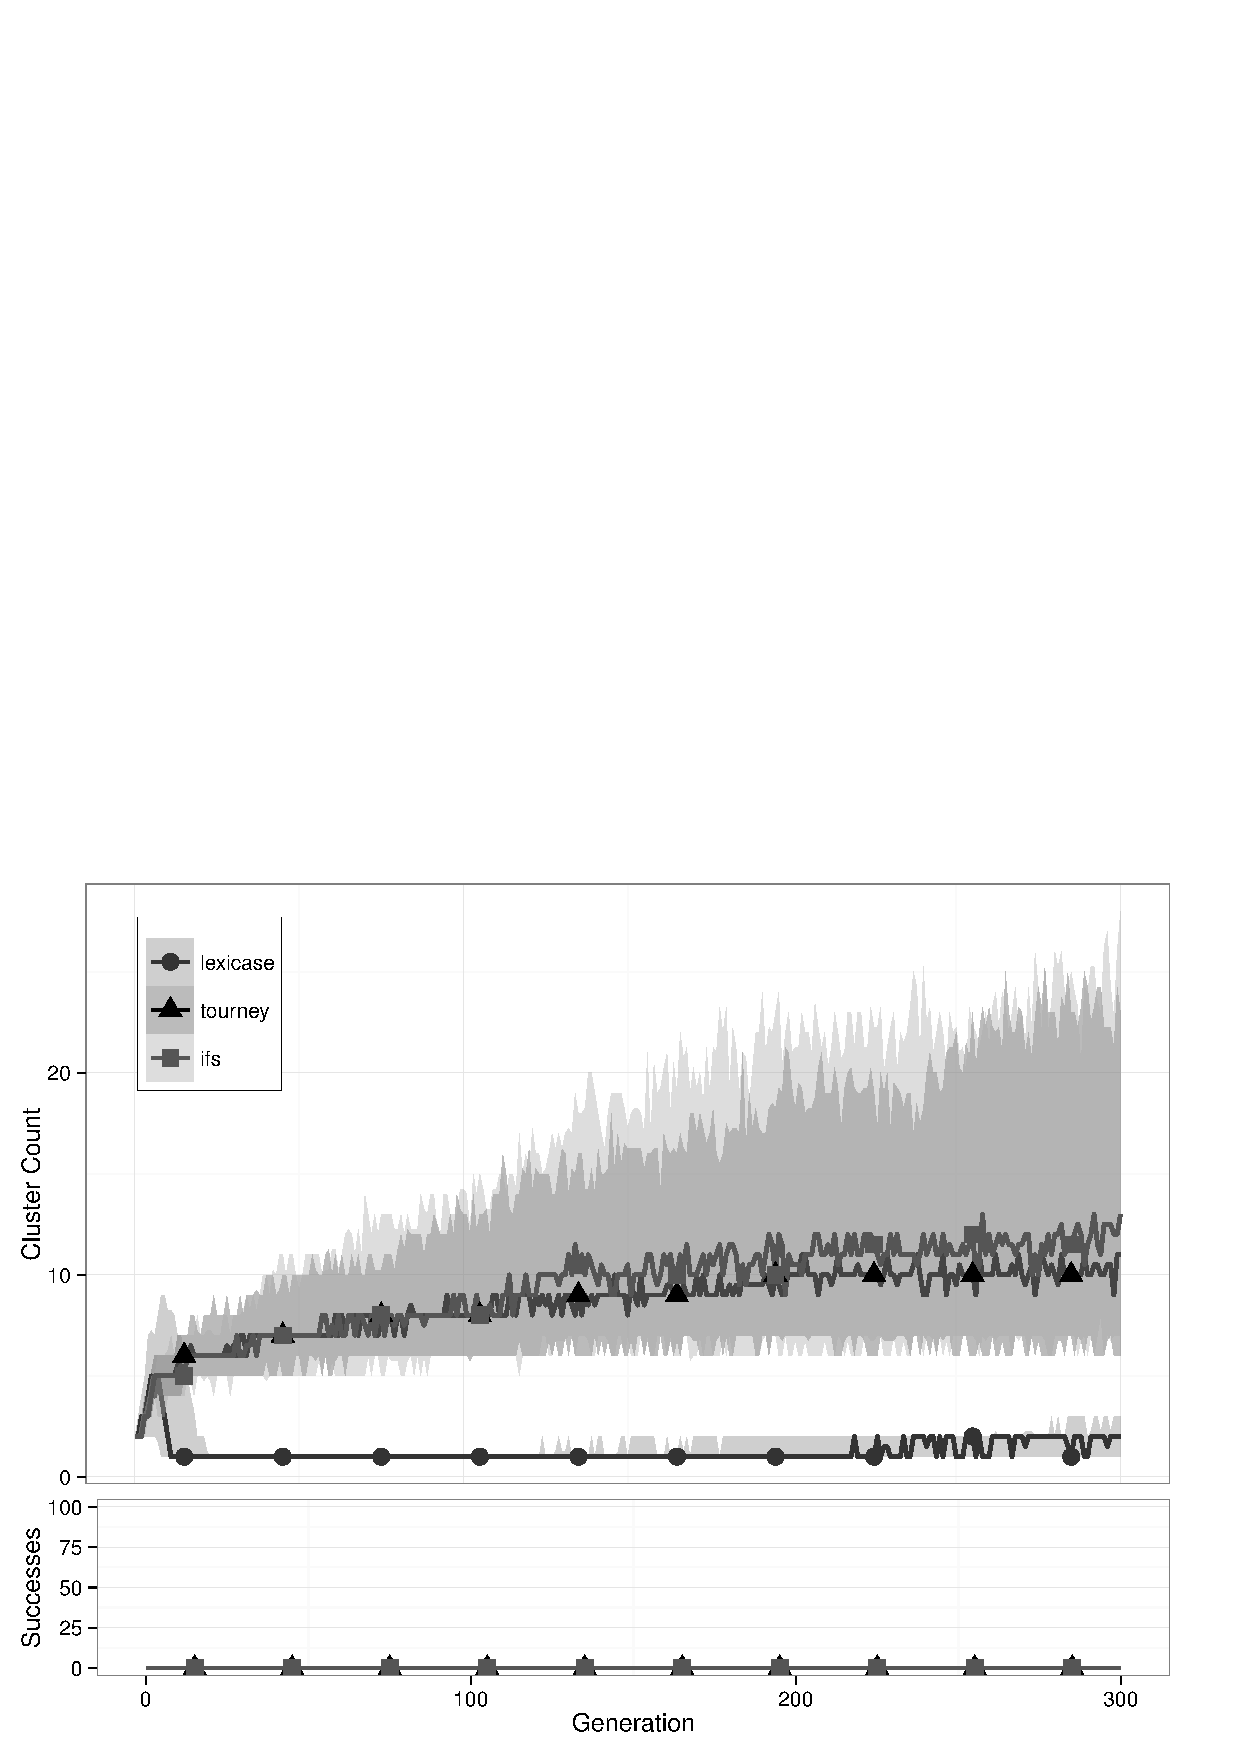
\includegraphics[width=11.5cm]{checksum-cluster.pdf}
\caption{checksum -- clusters.}
\label{checksumClu}
\end{figure}

\begin{figure}%[t] %[t] sets the image at the top of the page; t = top, b = bottom, h = here%
%\sidecaption[t]
\centering
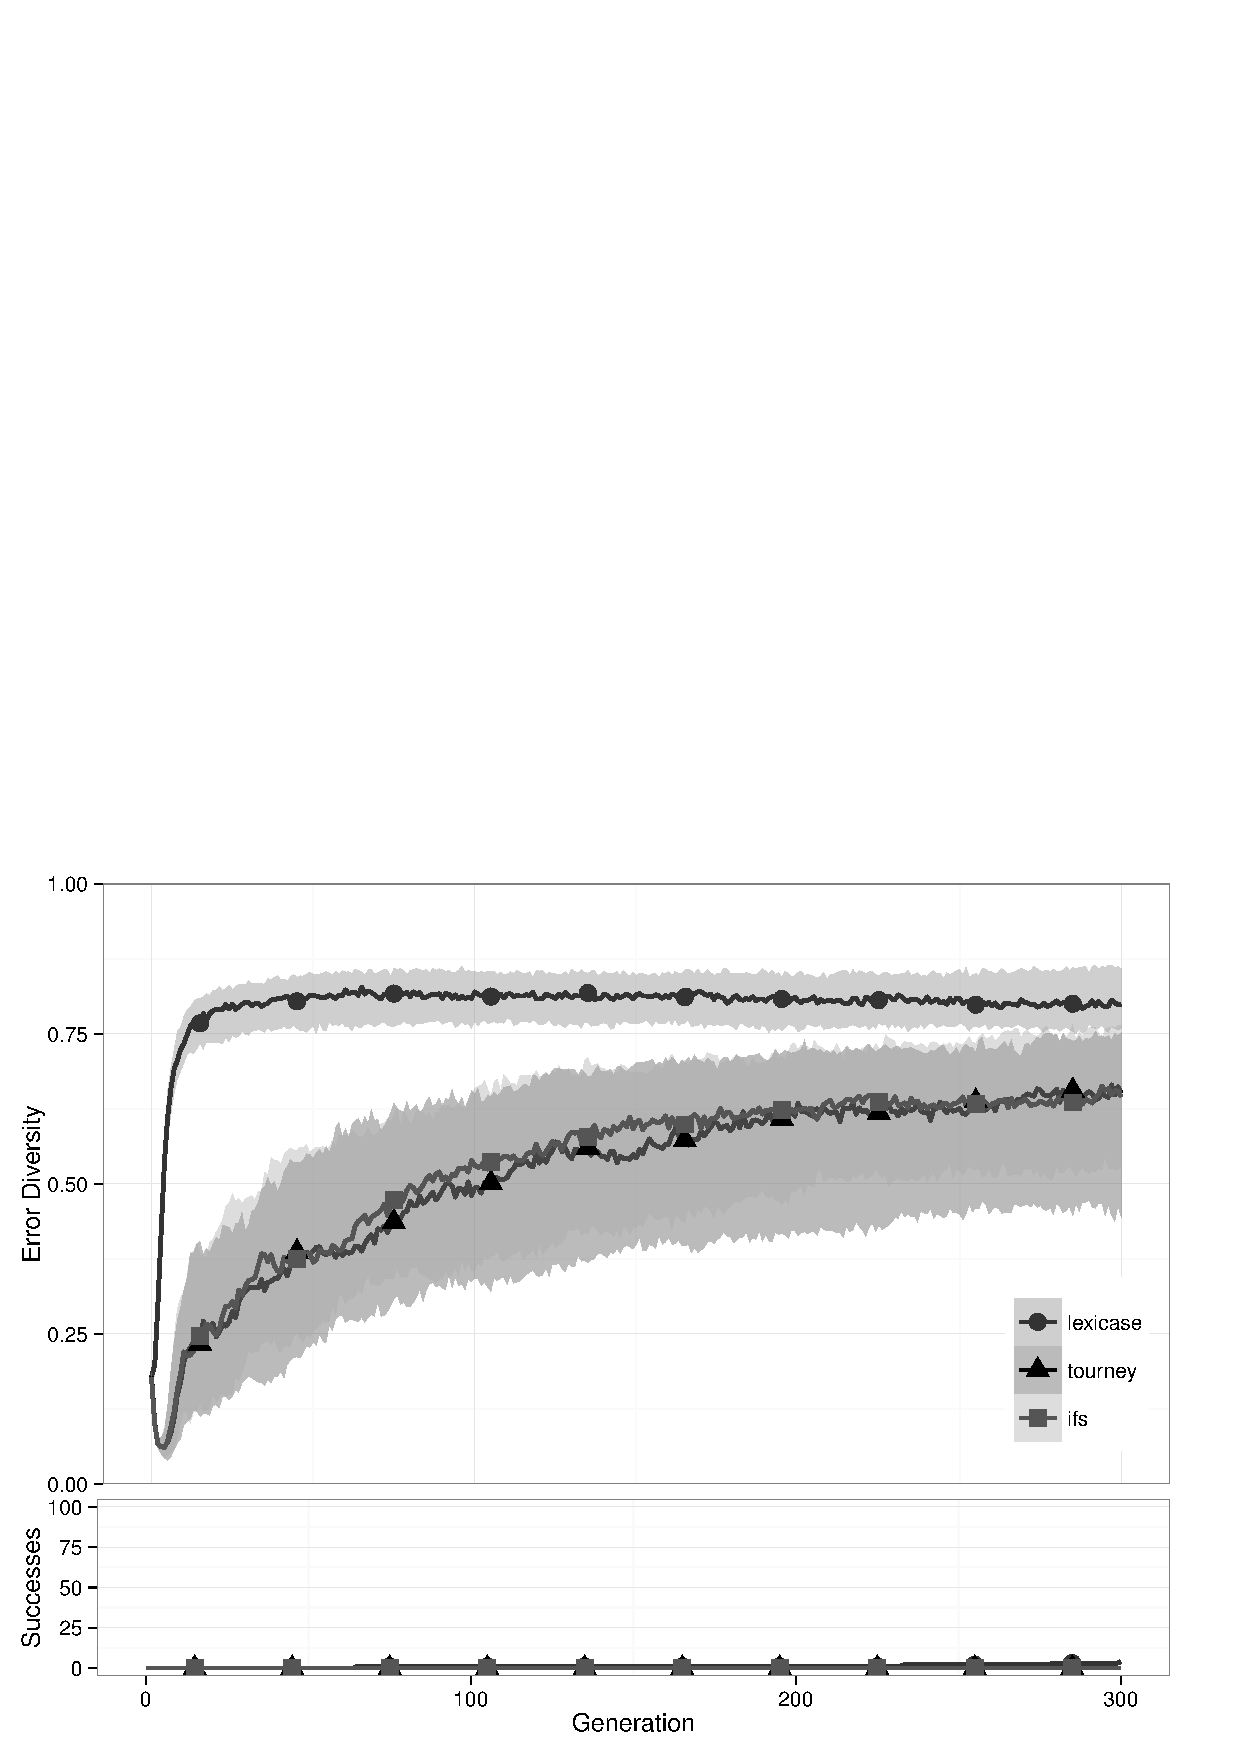
\includegraphics[width=11.5cm]{count-odds-diversity.pdf}
\caption{count-odds -- error diversity.}
\label{count-oddsDiv}
\end{figure}

\begin{figure}%[t] %[t] sets the image at the top of the page; t = top, b = bottom, h = here%
%\sidecaption[t]
\centering
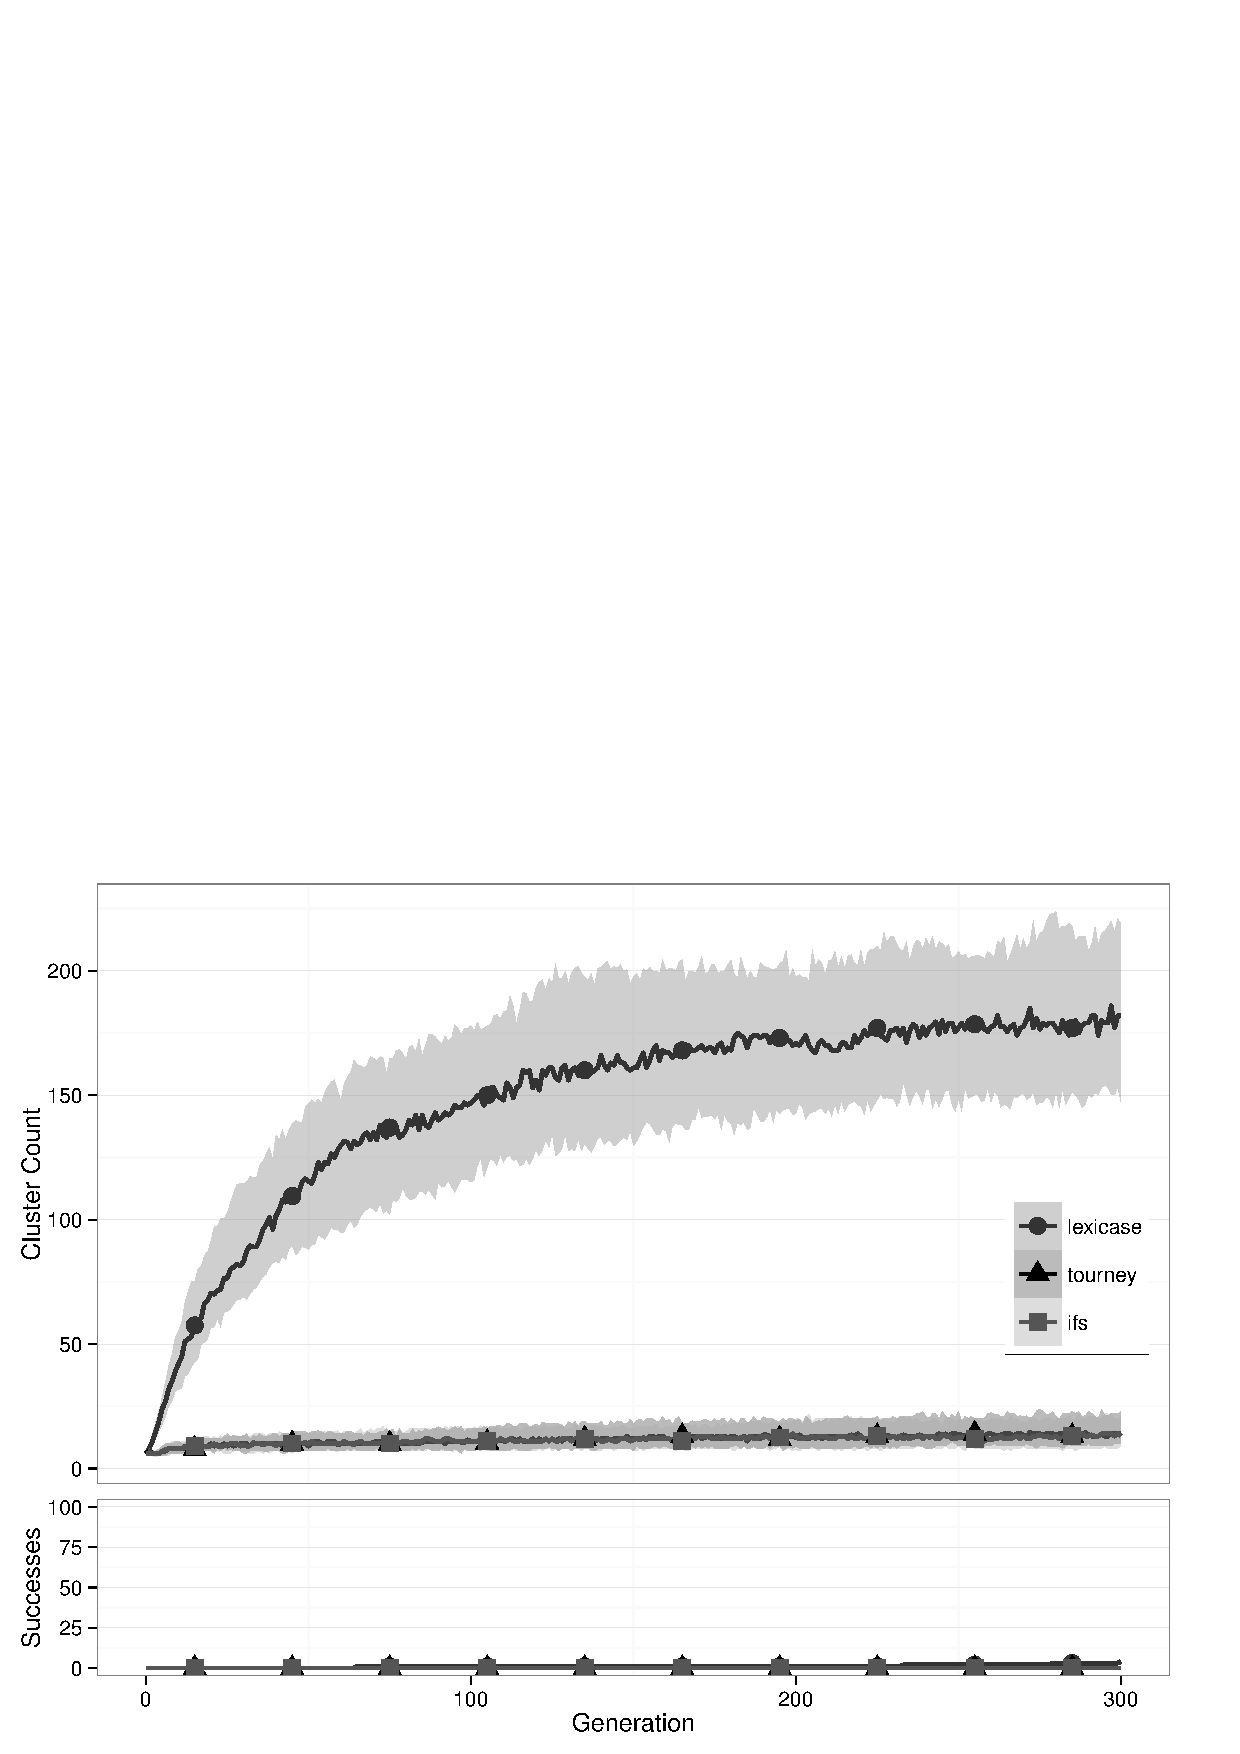
\includegraphics[width=11.5cm]{count-odds-cluster.pdf}
\caption{count-odds -- clusters.}
\label{count-oddsClu}
\end{figure}


\section{Discussion and importance of findings}

(include correlation with better success rates with lexicase)

\section{Conclusions}


\begin{acknowledgement}
Added later.
\end{acknowledgement}

\bibliographystyle{spbasic}
\bibliography{gp-bibliography,spector}
